\begin{enumerate}[label=\thechapter.\arabic*,ref=\thechapter.\theenumi]

\item Consider a unity-gain negative feedback system consisting of the plant $G\brak{s}$  and a proportional-integral controller. Let the proportional gain and integral
gain be 3 and 1, respectively. For a unit step reference input, the final values of the
controller output and the plant output, respectively, are
\begin{align}
    G\brak{s} = \frac{1}{\brak{s-1}} \notag
\end{align}\hfill (GATE EE 2023)\\
\solution 
\iffalse
\let\negmedspace\undefined
\let\negthickspace\undefined
\documentclass[journal,12pt,twocolumn]{IEEEtran}
\usepackage{cite}
\usepackage{amsmath,amssymb,amsfonts,amsthm}
\usepackage{algorithmic}
\usepackage{graphicx}
\usepackage{textcomp}
\usepackage{xcolor}
\usepackage{txfonts}
\usepackage{listings}
\usepackage{enumitem}
\usepackage{mathtools}
\usepackage{float}
\usepackage{gensymb}
\usepackage{comment}
\usepackage[breaklinks=true]{hyperref}
\usepackage{tkz-euclide} 
\usepackage{listings}
\usepackage{gvv}                                        
\def\inputGnumericTable{}                                 
\usepackage[latin1]{inputenc}                                
\usepackage{color}                                            
\usepackage{array}          
\usetikzlibrary{positioning, arrows.meta}
\usepackage{longtable}                                       
\usepackage{calc}                                             
\usepackage{multirow}                                         
\usepackage{hhline}                                           
\usepackage{ifthen}                                           
\usepackage{lscape}
\usepackage{amsmath}
\newtheorem{theorem}{Theorem}[section]
\newtheorem{problem}{Problem}
\newtheorem{proposition}{Proposition}[section]
\newtheorem{lemma}{Lemma}[section]
\newtheorem{corollary}[theorem]{Corollary}
\newtheorem{example}{Example}[section]
\newtheorem{definition}[problem]{Definition}
\newcommand{\BEQA}{\begin{eqnarray}}
\newcommand{\EEQA}{\end{eqnarray}}
\newcommand{\define}{\stackrel{\triangle}{=}}
\theoremstyle{remark}
\newtheorem{rem}{Remark}
\begin{document}

\bibliographystyle{IEEEtran}
\title{GATE-EE-Q14}
\author{EE23BTECH11015 - DHANUSH V NAYAK$^{*}$% <-this % stops a space
}
\maketitle
\newpage
\bigskip
\renewcommand{\thefigure}{\arabic{figure}}
\renewcommand{\thetable}{\theenumi}
\textbf{Question:}Consider a unity-gain negative feedback system consisting of the plant $G\brak{s}$  and a proportional-integral controller. Let the proportional gain and integral
gain be 3 and 1, respectively. For a unit step reference input, the final values of the
controller output and the plant output, respectively, are
\begin{align}
    G\brak{s} = \frac{1}{\brak{s-1}} \notag
\end{align}
\solution 
\fi
\begin{table}[H]
\centering
\renewcommand\thetable{1}
\setlength{\extrarowheight}{9pt}
\resizebox{0.5\textwidth}{!}{
\begin{tabular}{|c|c|c|}
\hline
\textbf{Parameter} & \textbf{Description} & \textbf{Value} \\ \hline
$K_{p}$ & Proportional Gain & 3  \\ \hline
$K_{i}$ & Integral Gain &1 \\ \hline
$r\brak{t}$& Reference Input & $u\brak{t}$ \\ \hline 
$w\brak{t}$& Controller Output & $?$ \\ \hline 
$y\brak{t}$ & Plant Output & $?$ \\ \hline
$e\brak{t}$ & Error Input & $r\brak{t}-y\brak{t}$ \\ \hline
\end{tabular}}
\caption{Parameter Table}
\label{tab:gate_ee_Q14}
\end{table}

From the\figref{fig:gate_ee_Q14_blockdiagram}:
\begin{align}
    E\brak{s}&= U\brak{s} - Y\brak{s}\label{eq:gate_ee_Q14.1}\\
W\brak{s} &= 3E\brak{s} + \frac{1}{s}E\brak{s}\label{eq:gate_ee_Q14.2}\\
    Y\brak{s} &= G\brak{s}W\brak{s} \label{eq:gate_ee_Q14.3}
\end{align}
Some results:
\begin{align}
    tx\brak{t} &\system{L} -\frac{d{X\brak{s}}}{ds} \label{eq:laplace_diff_prop}\\
    e^{-at}x\brak{t} &\system{L} X\brak{s+a}\label{eq:laplace_timeshifting_prop}
\end{align}
By using \eqref{eq:laplace_diff_prop} and \eqref{eq:laplace_timeshifting_prop}:
\begin{align}
    e^{-t}u\brak{t} &\system{L} \frac{1}{s+1} ,  Re\brak{s}>-1 \label{eq:gate_ee_Q14result.1}\\
    t e^{-t}u\brak{t} &\system{L} \frac{1}{\brak{s+1}^2},  Re\brak{s}>-1 
 \label{eq:gate_ee_Q14result.2}
\end{align}

\begin{figure}[H]
    \resizebox{0.9\textwidth}{!}{\tikzset{
    block/.style = {draw, fill=white, rectangle, minimum height=3em, minimum width=3em},
    tmp/.style  = {coordinate}, 
    minus/.style= {draw, fill=white, circle, node distance=1cm, append after command={\pgfextra \draw ($(\tikzlastnode.center) + (-0.15,0)$) -- ($(\tikzlastnode.center) + (0.15,0)$) node[above] {$-$}; \endpgfextra}},
    plus/.style= {draw, fill=white, circle, node distance=1cm, append after command={\pgfextra \draw ($(\tikzlastnode.center) + (-0.15,0)$) -- ($(\tikzlastnode.center) + (0.15,0)$) node[above] {$+$}; \endpgfextra}},
    input/.style = {coordinate},
    output/.style= {coordinate},
    pinstyle/.style = {pin edge={to-,thin,black}}
}


\begin{tikzpicture}[auto, node distance=2cm,>=latex]
    \node [input, name=rinput] (rinput) {};
    \node [minus, right of=rinput] (sum1) {};
    
    \node [block, right of=sum1] (controller) {$k_{p}=3$};
    \node [block, above of=controller, node distance=2cm] (up) {$\frac{k_{i}}{s}=\frac{3}{s}$};
    
    \node [plus, right of=controller, node distance=2cm] (sum2) {};
    \node [block, right of=sum2, node distance=3.5cm] (system) {$G\brak{s}=\frac{1}{\brak{s-1}}$};
    \node [output, right of=system, node distance=2cm] (output) {};
    \node [tmp, below of=controller] (tmp1) {$H(s)$};

    \draw [->] (rinput) -- node[below]{$r\brak{t}$} (sum1);
    \draw [->] (sum1) -- node[name=z,anchor=north,fill=white,circle,inner sep=1pt]{$e\brak{t}$} (controller);
    \draw [->] (controller) -- (sum2);
    \draw [->] (sum2) -- node[above, pos=0.8]{$w\brak{t}$} (system);
    \draw [->] (system) -- node [name=y] {$y\brak{t}$} (output);
    \draw [->] (z) |- (up);
    \draw [->] (up) -| (sum2);
    \draw [->] (y) |- (tmp1) -| (sum1);
\end{tikzpicture}
}
    \caption{Block Diagram of System}
    \label{fig:gate_ee_Q14_blockdiagram}
\end{figure}
\begin{enumerate}
\item \textbf{Plant Output:}\\
From \eqref{eq:gate_ee_Q14.1} , \eqref{eq:gate_ee_Q14.2} and \eqref{eq:gate_ee_Q14.3}:
\begin{align}
    Y\brak{s} &=  \frac{3s+1}{s\brak{s+1}^2} ,  Re\brak{s}>-1 \label{eq:Y(s)}
\end{align}
Final Value Theorem:    
\begin{align}
    \lim_{t \to \infty} x\brak{t}&= \lim_{s \to 0} sX\brak{s}\label{eq:finalval_thm}
\end{align}
Using \eqref{eq:finalval_thm} on Y\brak{s}:
\begin{align}
     \lim_{t \to \infty} y\brak{t}&= \lim_{s \to 0} sY\brak{s}\\
                            &= 1
\end{align}

Taking partial fraction of \eqref{eq:Y(s)} :
\begin{align}
    Y\brak{s} &= \frac{1}{s} + \frac{2}{\brak{s+1}^2} - \frac{1}{s+1}
\end{align}
Using \eqref{eq:gate_ee_Q14result.1} and \eqref{eq:gate_ee_Q14result.2}:
\begin{align}
    \therefore y\brak{t} &= u\brak{t}+ 2t e^{-t}u\brak{t} - e^{-t}u\brak{t}
\end{align}
\item \textbf{Controller Output:}\\
From \eqref{eq:gate_ee_Q14.2}
\begin{align}
     W\brak{s} &= \frac{3}{s} + \frac{1}{s^2} - Y\brak{s}\brak{3+\frac{1}{s}}
\end{align}
Substituting \eqref{eq:Y(s)}
\begin{align}
    W\brak{s} &= \frac{\brak{s-1}\brak{3s+1}}{s\brak{s+1}^2} ,  Re\brak{s}>-1 \label{eq:W(s)}
\end{align}
Using \eqref{eq:finalval_thm} on W\brak{s}
\begin{align}
     \lim_{t \to \infty} w\brak{t}&= \lim_{s \to 0} sW\brak{s}\\
                            &= -1
\end{align}
Taking partial fraction of equation\eqref{eq:W(s)} :
\begin{align}
    W\brak{s} &= -\frac{1}{s} - \frac{4}{\brak{s+1}^2} + \frac{4}{s+1}
\end{align}
Using equations \eqref{eq:gate_ee_Q14result.1} and \eqref{eq:gate_ee_Q14result.2} and taking inverse lapalace transform:
\begin{align}
    w\brak{t} &= -u\brak{t}-4t e^{-t}u\brak{t} +4 e^{-t}u\brak{t}
\end{align}

\begin{figure}[H]
    \includegraphics[width=1\columnwidth]{2023/EE/14/figs/Plot of w(t).png}
    \caption{$w\brak{t}$ converges at -1.}
    \label{fig:w_t}
\end{figure}

\begin{figure}[H]
    \includegraphics[width=1\columnwidth]{2023/EE/14/figs/Plot of y(t).png}
    \caption{$y\brak{t}$ converges at +1}
    \label{fig:y_t}
\end{figure}

\end{enumerate}
%\end{document}


\newpage

\item Level \brak{h} in a steam boiler is controlled by manipulating the flow rate \brak{F} of the break-up(fresh) water using a proportional \brak{P} controller. The transfer function between the output and the manipulated input is   \\
$$ \frac{h\brak{s}}{F\brak{s}}=\frac{0.25\brak{1-s}}{s\brak{2s+1}} $$   \\
The measurement and the valve transfer functions are both equal to 1. A process engineer wants to tune the controller so that the closed loop response gives the decaying oscillations under the servo mode. Which one of the following is the CORRECT value of the controller gain to be used by the engineer? \\
\begin{enumerate}[label=(\alph*)]
    \item $0.25$
    \item $2$
    \item $4$
    \item $6$
\end{enumerate} \hfill{GATE CH 2023} \\

\solution
 \iffalse
\let\negmedspace\undefined
\let\negthickspace\undefined
\documentclass[journal,12pt,twocolumn]{IEEEtran}
\usepackage{cite}
\usepackage{amsmath,amssymb,amsfonts,amsthm}
\usepackage{algorithmic}
\usepackage{graphicx}
\usepackage{textcomp}
\usepackage{xcolor}
\usepackage{txfonts}
\usepackage{listings}
\usepackage{enumitem}
\usepackage{mathtools}
\usepackage{gensymb}
\usepackage{comment}
\usepackage[breaklinks=true]{hyperref}
\usepackage{tkz-euclide} 
\usepackage{listings}
\usepackage{gvv}                                        
\def\inputGnumericTable{}                                 
\usepackage[latin1]{inputenc}                                
\usepackage{color}                                            
\usepackage{array}                                            
\usepackage{longtable}                                       
\usepackage{calc}                                             
\usepackage{multirow}                                         
\usepackage{hhline}                                           
\usepackage{ifthen}                                           
\usepackage{lscape}

\newtheorem{theorem}{Theorem}[section]
\newtheorem{problem}{Problem}
\newtheorem{proposition}{Proposition}[section]
\newtheorem{lemma}{Lemma}[section]
\newtheorem{corollary}[theorem]{Corollary}
\newtheorem{example}{Example}[section]
\newtheorem{definition}[problem]{Definition}
\newcommand{\BEQA}{\begin{eqnarray}}
\newcommand{\EEQA}{\end{eqnarray}}
\newcommand{\define}{\stackrel{\triangle}{=}}
\theoremstyle{remark}
\newtheorem{rem}{Remark}
\begin{document}
\parindent 0px
\bibliographystyle{IEEEtran}
\title{GATE: CH - 45.2023}
\author{EE22BTECH11219 - Rada Sai Sujan$^{}$% <-this % stops a space
}
\maketitle
\newpage
\bigskip
\section*{Question}
Level \brak{h} in a steam boiler is controlled by manipulating the flow rate \brak{F} of the break-up(fresh) water using a proportional \brak{P} controller. The transfer function between the output and the manipulated input is   \\
$$ \frac{h\brak{s}}{F\brak{s}}=\frac{0.25\brak{1-s}}{s\brak{2s+1}} $$   \\
The measurement and the valve transfer functions are both equal to 1. A process engineer wants to tune the controller so that the closed loop response gives the decaying oscillations under the servo mode. Which one of the following is the CORRECT value of the controller gain to be used by the engineer? \\
\begin{enumerate}[label=(\alph*)]
    \item $0.25$
    \item $2$
    \item $4$
    \item $6$
\end{enumerate} \\
\solution
\fi

\begin{table}[ht]
    \centering
    \begin{tabular}{|p{2cm}|p{6cm}|}
    \hline
    PARAMETER & DESCRIPTION \\ \hline
    $$G_c$$ & Proportional controller's transfer function \\ \hline
    $$G_f$$ & Valve transfer function \\ \hline
    $$G_p$$ & Process transfer function   \\ \hline
    $$G_M$$ & Measurement transfer function \\ \hline 
    $$G\brak{s}$$ & Open loop transfer function \\ \hline
    $$T\brak{s}$$ & Transfer function of system \\ \hline
\end{tabular}

    \caption{PARAMETER TABLE 1}
    \label{tab:ch.45.1}
\end{table} 
\begin{figure}[ht]
    \centering
    \includegraphics[width=\columnwidth]{2023/CH/45/figs/k.png}
    \caption{Closed loop Block diagram}
    \label{fig:ch.45.1}
\end{figure}    
Closed loop signal transfer function of the above block diagram can be given by,
\begin{align}
     T\brak{s} &= \frac{G\brak{s}}{1+G\brak{s}H\brak{s}}    
\end{align}
From \figref{fig:ch.45.1} and \tabref{tab:ch.45.1}
for a unit impulse, $X\brak{s}=1$ \\
\begin{align}
    h\brak{s} &= T\brak{s}\times X\brak{s}   \\
    h\brak{s} &= \frac{\brak{1-s}K_c}{8s^2 + \brak{4-K_c}s + K_c}  \\
    \implies h\brak{s} &= \frac{\brak{1-s}K_c}{8\brak{s-s_1}\brak{s-s_2}}  \label{eq:ch.45.4}
\end{align}
Where,
\begin{align}
    s_1 &= \frac{\brak{K_c-4}}{16} + \sqrt{\brak{\frac{K_c-4}{16}}^2 - \frac{K_c}{8}}  \\
    s_2 &= \frac{\brak{K_c-4}}{16} - \sqrt{\brak{\frac{K_c-4}{16}}^2 - \frac{K_c}{8}} 
\end{align}
From \eqref{eq:ch.45.4} we get,
\begin{align}
    h\brak{s} &= \frac{K_c}{8\brak{s_1-s_2}}\brak{\frac{1-s_1}{s-s_1}-\frac{1-s_2}{s-s_2}}
\end{align}
Now taking the inverse laplace transform we have,
\begin{align}
    h\brak{t} &= \frac{K_c}{8\brak{s_1-s_2}} \left [\brak{1-s_1}e^{s_1t}-\brak{1-s_2}e^{s_2t} \right ]u\brak{t}  \\
    \implies h\brak{t} &= e^{\frac{K_c-4}{16}}\brak{A_1e^{\sqrt{\brak{\frac{K_c-4}{16}}^2 - \frac{K_c}{8}}} - A_2e^{-\sqrt{\brak{\frac{K_c-4}{16}}^2 - \frac{K_c}{8}}}}u\brak{t}    
\end{align}
Where,
\begin{align}
    A_1 &= \frac{K_c}{8} \brak{\frac{1-s_1}{s_1-s_2}}    \\
    A_2 &= \frac{K_c}{8} \brak{\frac{1-s_2}{s_1-s_2}}    
\end{align}
Now applying the condition for underdamped oscillations,
\begin{align}
    \brak{\frac{K_c-4}{16}}^2 - \frac{K_c}{8} < 0    \\
    \implies K_c \in \brak{20-\sqrt{384} , 20+\sqrt{384}}   \label{eq:ch.45.13}
\end{align}
For the system to be stable,
\begin{align}
    \frac{K_c-4}{8}&<0   \\
    \implies K_c&<4 	\label{eq:ch.45.15}
\end{align}
From \eqref{eq:ch.45.13} and \eqref{eq:ch.45.15}
\begin{align}
    &K_c \in \brak{0.4,4}    \label{eq:ch.45.16}
\end{align}
\eqref{eq:ch.45.16} represents the $ROC$,$(R_e\{s\}<0)$
\begin{align}
    \implies &K_c=2
\end{align}
\begin{figure}[htbp]
    \centering
    \includegraphics[width=\columnwidth]{2023/CH/45/figs/b.png}
    \caption{y\brak{t} $vs$ t graph}
    \label{fig:ch.45.2}
\end{figure}     

\newpage
\item The figure shows a block of mass m = 20 kg attached to a pair of identical linear springs, each having a spring constant k = 1000 N/m. The block oscillates on a frictionless horizontal surface. Assuming free vibrations, the time taken by the block to complete ten oscillations is \rule{1cm}{0.15mm} seconds . (Rounded off to two decimal places) Take $\pi$ = 3.14. \\ \hfill(GATE ME 2023)

\begin{figure}[!ht]
\centering
\begin{center}
\includegraphics[width=\columnwidth]{2023/ME/30/figs/questiondiagram.jpg}
\end{center}
%\caption{Diagram for GATE ME Question 30}
\end{figure}
\solution
\iffalse
\let\negmedspace\undefined
\let\negthickspace\undefined
\documentclass[journal,12pt,twocolumn]{IEEEtran}
\usepackage{cite}
\usepackage{amsmath,amssymb,amsfonts,amsthm}
\usepackage{algorithmic}
\usepackage{graphicx}
\usepackage{textcomp}
\usepackage{xcolor}
\usepackage{txfonts}
\usepackage{listings}
\usepackage{enumitem}
\usepackage{mathtools}
\usepackage{gensymb}
\usepackage{comment}
\usepackage[breaklinks=true]{hyperref}
\usepackage{tkz-euclide} 
\usepackage{listings}
\usepackage{gvv}                                        
\def\inputGnumericTable{}                                 
\usepackage[latin1]{inputenc}                                
\usepackage{color}                                            
\usepackage{array}                                            
\usepackage{longtable}                                       
\usepackage{calc}                                             
\usepackage{multirow}                                         
\usepackage{hhline}                                           
\usepackage{ifthen}                                           
\usepackage{lscape}
\usepackage{placeins}
\usepackage{xparse}


\newtheorem{theorem}{Theorem}[section]
\newtheorem{problem}{Problem}
\newtheorem{proposition}{Proposition}[section]
\newtheorem{lemma}{Lemma}[section]
\newtheorem{corollary}[theorem]{Corollary}
\newtheorem{example}{Example}[section]
\newtheorem{definition}[problem]{Definition}
\newcommand{\BEQA}{\begin{eqnarray}}
\newcommand{\EEQA}{\end{eqnarray}}
\newcommand{\define}{\stackrel{\triangle}{=}}
\theoremstyle{remark}
\newtheorem{rem}{Remark}

\graphicspath{ {./figs/} } 

\begin{document}

\bibliographystyle{IEEEtran}
\vspace{3cm}

\Large\title{GATE ME 30}
\large\author{EE23BTECH11032 - Kaustubh Parag Khachane $^{*}$% <-this % stops a space
}
\maketitle
\newpage
\bigskip

\renewcommand{\thefigure}{\theenumi}
\renewcommand{\thetable}{\theenumi}
\large\textbf{Question GATE ME 30} :\\
The figure shows a block of mass m = 20 kg attached to a pair of identical linear springs, each having a spring constant k = 1000 N/m. The block oscillates on a frictionless horizontal surface. Assuming free vibrations, the time taken by the block to complete ten oscillations is \rule{1cm}{0.15mm} seconds . (Rounded off to two decimal places) Take $\pi$ = 3.14. \\ \hfill(GATE ME 2023)

\begin{figure}[!ht]
\centering
\begin{center}
\includegraphics[width=\columnwidth]{2023/ME/30/figs/questiondiagram.jpg}
\end{center}
%\caption{Diagram for GATE ME Question 30}
\end{figure}

\solution\\
\fi
\begin{table}[!ht] 
\centering
\setlength{\extrarowheight}{8pt}
\begin{tabular}{|l|l|l|}
    \hline
    \textbf{Parameter} & \textbf{Description} & \textbf{Value} \\
    \hline
     $k_i$ & spring constant & 1000 N/m \\
    \hline
     m & mass of block & 20Kg \\
    \hline
    k & Equivalent spring constant& $k_1 + k_2$ (parallel)\\
    \hline
     $\omega_n$ & Natural frequency & $\sqrt{\frac{k}{m}}$ \\
    \hline
    T & Time period of an oscillation & $\frac{2\pi}{\omega_n}$ \\
    \hline
    x & Displacement of block & \\
    \hline
    a & Acceleration of block & $\frac{d^2x}{dt^2}$\\
    \hline
    F & Force on block & \\
    \hline
    A & Amplitude of oscillation & x\brak{0}\\
    \hline
  \end{tabular}
  \vspace{4mm}
 \caption{Parameter Table}
 \label{tab:table0_me30_2023}
\end{table}

\begin{align}
    F &= ma \\
    F &= -kx \\
    \implies ma + kx &= 0\\
    \therefore m\frac{d^2x}{dt^2} + kx &= 0\label{eq:eq1_me30_2023}
\end{align}
The Laplace transform of the terms is ,
\begin{align}
    x & \system{\mathcal{L}} X\brak{s}\label{eq:eq3_me30_2023}\\
    \frac{d^2x}{dt^2} & \system{\mathcal{L}} s^2 X\brak{s} - sx\brak{0} - \dot{x}\brak{0}\label{eq:eq2_me30_2023}
\end{align}
Using equation \eqref{eq:eq3_me30_2023} and \eqref{eq:eq2_me30_2023} in equation \eqref{eq:eq1_me30_2023},
\begin{align}
    &m\brak{s^2 X\brak{s} - sx\brak{0} - \dot{x}\brak{0}} + kX\brak{s} = 0\\
    &ms^2X\brak{s} -msA + kX\brak{s} = 0
\end{align}
\begin{align}
    X\brak{s} &= \frac{msA}{ms^2 + k} \\
     &= \frac{sA}{s^2 + \frac{k}{m}} \label{eq:eq4_me30_2023}
\end{align}
The inverse Laplace transform of such terms is given by,
\begin{align}
    \frac{s}{s^2 + a^2} \system{\mathcal{L^{ -}}} cos\brak{at}u\brak{t}
\end{align}
$\therefore$ the inverse Laplace of \eqref{eq:eq4_me30_2023} is,
\begin{align}
    x\brak{t} = Acos\brak{\sqrt{\frac{k}{m}}t} \label{eq:eq5_me30_2023}
\end{align}
From equation \eqref{eq:eq5_me30_2023} and \tabref{tab:table0_me30_2023} ,the time to complete one oscillation is,
\begin{align}
    T_n &= \frac{2\pi}{\sqrt{\frac{k}{m}}}\\
    &= \frac{\pi}{5}\label{eq:eq6_me30_2023}
\end{align}
$\therefore$ the time required for 10 oscillations is ,
\begin{align}
    10T_n &= 2\pi\\
    &= 6.28 s
\end{align}
\begin{figure}[!ht]
\centering
\begin{center}
\includegraphics[width=\columnwidth]{2023/ME/30/figs/Figure_1.png}
\end{center}
\caption{Plot of $x\brak{t}$}
\end{figure}

\newpage

\item A system has transfer function
 \[\frac{Y(s)}{X(s)}=\frac {s-\pi}{s+\pi}\]
 let $u(t)$ be the unit step function.The input $x(t)$ that results in a steady-state output $y(t)=sin(\pi t)$ is \underline{\quad}.\hfill (GATE IN 2023)\\
 \solution
 \documentclass[journal,12pt,twocolumn]{IEEEtran}
\usepackage{cite}
\usepackage{amsmath,amssymb,amsfonts,amsthm}
\usepackage{algorithmic}
\usepackage{graphicx}
\usepackage{textcomp}
\usepackage{xcolor}
\usepackage{txfonts}
\usepackage{listings}
\usepackage{enumitem}
\usepackage{mathtools}
\usepackage{gensymb}
\usepackage{comment}
\usepackage[breaklinks=true]{hyperref}
\usepackage{tkz-euclide} 
\usepackage{listings}
\usepackage{gvv}                                        
\def\inputGnumericTable{}                                 
\usepackage[latin1]{inputenc}                                
\usepackage{color}                                            
\usepackage{array}                                            
\usepackage{longtable}                                       
\usepackage{calc}                                             
\usepackage{multirow}                                         
\usepackage{hhline}                                           
\usepackage{ifthen}                                           
\usepackage{lscape}
\usepackage{caption}
\usepackage{subfigure}

% Define \phase command
\newcommand{\phase}[1]{\text{arg}\left(#1\right)}

\newtheorem{theorem}{Theorem}[section]
\newtheorem{problem}{Problem}
\newtheorem{proposition}{Proposition}[section]
\newtheorem{lemma}{Lemma}[section]
\newtheorem{corollary}[theorem]{Corollary}
\newtheorem{example}{Example}[section]
\newtheorem{definition}[problem]{Definition}
\newcommand{\BEQA}{\begin{eqnarray}}
\newcommand{\EEQA}{\end{eqnarray}}
\newcommand{\system}[1]{\stackrel{#1}{\rightarrow}}
\newcommand{\define}{\stackrel{\triangle}{=}}
\theoremstyle{remark}
\newtheorem{rem}{Remark}

\begin{document}

\bibliographystyle{IEEEtran}
\vspace{3cm}

\title{Gate.in.21}
\author{EE22BTECH11008 - Annapureddy Siva Meenakshi$^{*}$}
\maketitle
\bigskip

\renewcommand{\thefigure}{\theenumi}
\renewcommand{\thetable}{\theenumi}
Q: A system has transfer function
\[\frac{Y(s)}{X(s)}=\frac {s-\pi}{s+\pi}\]
let $u(t)$ be the unit step function. The input $x(t)$ that results in a steady-state output $y(t)=\sin(\pi t)$ is \underline{\quad}.
\solution

\begin{figure}[htb]
  \centering
  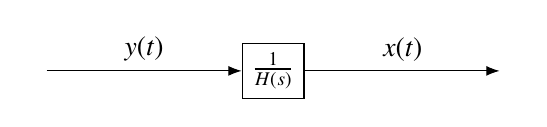
\begin{tikzpicture}[auto, node distance=4cm,>={Latex}]
  % Define blocks
  \node (input) at (0,0) {};
  \node [draw, rectangle] (H) at (3,0) {$\frac{1}{H(s)}$}; 
  \node (output) at (6,0) {};

  % Connect blocks with right arrows
  \draw [->] (input) -- node[midway, above] {$y(t)$} (H);
  \draw [->] (H) -- node[midway, above] {$x(t)$} (output);
\end{tikzpicture}

  \captionsetup{justification=centering, singlelinecheck=off}
  \caption{Block diagram of the inverse system}
  \label{fig:in_21_f1}
\end{figure}

\begin{figure}[htb]
  \centering
  \documentclass{standalone}
\usepackage{circuitikz}
\usepackage{siunitx}

\begin{document}
\begin{circuitikz}
    \draw (0,3) to[R, l=\SI{3}{\kohm}, i=$I$] (4,3);
    \draw (4,3) to[R, l=\SI{10}{\kohm}, i=$I_2$] (8,3);
    \draw (0,3) to[battery1, v=$\frac{10}{s}\si{\volt}$, american] (0,0);
    \draw (4,3) to[R, l=\SI{7}{\kohm}, i=$I_1$] (4,0);
    \draw (8,3) to[C, l=$\frac{1}{Cs}$, v=$V_c(s)$, american] (8,0);
    \draw (0,0) to (8,0);
\end{circuitikz}
\end{document}


  \captionsetup{justification=centering, singlelinecheck=off}
  \caption{Block diagram of the system}
  \label{fig:in_21_f2}
\end{figure}

\begin{table}[!ht]
    \centering
        \begin{tabular}{|c|c|c|}
\hline
\textbf{Parameter} & \textbf{Description} & \textbf{Value}\\ \hline
$Y\brak{s}$ & Output node variable &\\ \hline
$R\brak{s}$ & Input node variable &\\ \hline
$\frac{Y\brak{s}}{R\brak{s}}$ & Transfer function & ?\\ \hline
$P_1$ & Forward path gain a-b-c & $\frac{2}{s}$ \\ \hline
$P_2$ & Forward path gain a-c & $3$ \\ \hline
$\Delta_1$ & Determinant of forward path a-b-c & $1$ \\ \hline
$\Delta_2$ & Determinant of forward path a-c & $1$ \\ \hline
$\Delta$ & Determinant of system & $1-\frac{1}{s}$ \\ \hline
$n$ & Number of forward path & $2$ \\ \hline
\end{tabular}

    \caption{Input parameters}
    \label{tab:in_21_t1}
\end{table}

\begin{equation}
    H(s) = \frac{s - \pi}{s + \pi} 
\end{equation}
from ~\figref{fig:in_21_f1}
\begin{equation}
	\frac{1}{H(s)} = \frac{s + \pi}{s - \pi}
\end{equation}
Converting transfer function to frequency response, we get
\begin{equation}
    \frac{1}{H(j\omega)}=\frac{j\omega+\pi}{j\omega-\pi}
\end{equation}
from ~\tabref{tab:in_21_t1} $\omega=\pi$
\begin{equation}
   \frac{1}{H(j\pi)} = \frac{j + 1}{j - 1} = -j = e^{-j\frac{\pi}{2}}\label{eq:in.21.4} 
\end{equation}
from ~\eqref{eq:in.21.4} 
\begin{equation}
	\abs{\frac{1}{H(j\pi)}}=1 \quad \text{and} \quad \phase{\frac{1}{H(j\pi)}} = -90^\circ
\end{equation}
\begin{equation}
    y(t) = \sin(\pi t) \label{eq:in.21.6}
\end{equation}

\begin{align}
  \sin(\pi t)&\system{\frac{1}{H(j\omega)}}\abs{\frac{1}{H(j\omega)}}\sin\left(\pi t  + \phase{\frac{1}{H(j\omega)}}\right)\label{eq:in.21.8}
\end{align}

Therefore, by ~\eqref{eq:in.21.6} and ~\eqref{eq:in.21.8}, we get
\begin{equation}
    x(t)=\sin\left(\pi t -\frac{\pi}{2}\right)
\end{equation}

\begin{figure}[h]
  \centering
  \includegraphics[width=\columnwidth]{./figs/figure3.png} 
  \captionsetup{justification=centering}
  \caption{Plot of $x(t)$ and $y(t)$ taken from Python}
  \label{fig:in.21.f3}
\end{figure}

\begin{figure}[h]
  \centering

  \subfigure[Amplitude of $\frac{1}{H(j\omega)}$]{
    \includegraphics[width=0.45\linewidth]{./figs/figure1.png}
    \label{fig:in.21.subfig.1}
  }
  \hfill
  \subfigure[Phase of $\frac{1}{H(j\omega)}$]{
    \includegraphics[width=0.45\linewidth]{./figs/figure2.png}
    \label{fig:in.21.subfig.2}
  }
  \caption{Amplitude and Phase of $\frac{1}{H(j\omega)}$}
  \label{fig:in.21.subfig}
\end{figure}

\end{document}


 \newpage

\item Consider the complex function
\[ f(z) = \frac{z^{2}\sin z}{(z-\pi)^4} \]
At \( z = \pi \), which of the following options is (are) correct?
\begin{enumerate}[label=\textbf{\arabic*.}, font=\bfseries, align=left]
    \item[(A)] The order of the pole is 4 
    \item[(B)] The order of the pole is 3 
    \item[(C)] The residue at the pole is \( \frac{\pi}{6} \)
    \item[(D)] The residue at the pole is \( \frac{2\pi}{3} \)
\end{enumerate}
\hfill (GATE PH 2023)
\solution
\iffalse
\let\negmedspace\undefined
\let\negthickspace\undefined
\documentclass[journal,12pt,onecolumn]{IEEEtran}
\usepackage{cite}
\usepackage{amsmath,amssymb,amsfonts,amsthm}

\usepackage{graphicx}
\usepackage{textcomp}
\usepackage{xcolor}
\usepackage{txfonts}
\usepackage{listings}
\usepackage{enumitem}
\usepackage{mathtools}
\usepackage{gensymb}
\usepackage[breaklinks=true]{hyperref}
\usepackage{tkz-euclide} % loads  TikZ and tkz-base
\usepackage{listings}
\usepackage{gvv}
\usepackage{booktabs}

%
%\usepackage{setspace}
%\usepackage{gensymb}
%\doublespacing
%\singlespacing

%\usepackage{graphicx}
%\usepackage{amssymb}
%\usepackage{relsize}
%\usepackage[cmex10]{amsmath}
%\usepackage{amsthm}
%\interdisplaylinepenalty=2500
%\savesymbol{iint}
%\usepackage{txfonts}
%\restoresymbol{TXF}{iint}
%\usepackage{wasysym}
%\usepackage{amsthm}
%\usepackage{iithtlc}
%\usepackage{mathrsfs}
%\usepackage{txfonts}
%\usepackage{stfloats}
%\usepackage{bm}
%\usepackage{cite}
%\usepackage{cases}
%\usepackage{subfig}
%\usepackage{xtab}
%\usepackage{longtable}
%\usepackage{multirow}

%\usepackage{algpseudocode}
%\usepackage{enumitem}
%\usepackage{mathtools}
%\usepackage{tikz}
%\usepackage{circuitikz}
%\usepackage{verbatim}
%\usepackage{tfrupee}
%\usepackage{stmaryrd}
%\usetkzobj{all}
%    \usepackage{color}                                            %%
%    \usepackage{array}                                            %%
%    \usepackage{longtable}                                        %%
%    \usepackage{calc}                                             %%
%    \usepackage{multirow}                                         %%
%    \usepackage{hhline}                                           %%
%    \usepackage{ifthen}                                           %%
  %optionally (for landscape tables embedded in another document): %%
%    \usepackage{lscape}     
%\usepackage{multicol}
%\usepackage{chngcntr}
%\usepackage{enumerate}

%\usepackage{wasysym}
%\documentclass[conference]{IEEEtran}
%\IEEEoverridecommandlockouts
% The preceding line is only needed to identify funding in the first footnote. If that is unneeded, please comment it out.

\newtheorem{theorem}{Theorem}[section]
\newtheorem{problem}{Problem}
\newtheorem{proposition}{Proposition}[section]
\newtheorem{lemma}{Lemma}[section]
\newtheorem{corollary}[theorem]{Corollary}
\newtheorem{example}{Example}[section]
\newtheorem{definition}[problem]{Definition}
%\newtheorem{thm}{Theorem}[section] 
%\newtheorem{defn}[thm]{Definition}
%\newtheorem{algorithm}{Algorithm}[section]
%\newtheorem{cor}{Corollary}
\newcommand{\BEQA}{\begin{eqnarray}}
\newcommand{\EEQA}{\end{eqnarray}}
\newcommand{\define}{\stackrel{\triangle}{=}}
\theoremstyle{remark}
\newtheorem{rem}{Remark}

%\bibliographystyle{ieeetr}
\begin{document}
%

\bibliographystyle{IEEEtran}


\vspace{3cm}

\title{
%	\logo{
Gate Question

\large{EE:1205 Signals and Systems}

Indian Institute of Technology, Hyderabad
%	}
}
\author{Abhey Garg

EE23BTECH11202
}	


% make the title area
\maketitle


%\tableofcontents

\bigskip

\renewcommand{\thefigure}{\arabic{figure}}
\renewcommand{\thetable}{\arabic{table}}
\renewcommand{\theequation}{\arabic{equation}}

\section{Question GATE PH 56}
Consider the complex function
\[ f(z) = \frac{z^{2}\sin z}{(z-\pi)^4} \]
At \( z = \pi \), which of the following options is (are) correct?
\begin{enumerate}[label=\textbf{\arabic*.}, font=\bfseries, align=left]
    \item[(A)] The order of the pole is 4 
    \item[(B)] The order of the pole is 3 
    \item[(C)] The residue at the pole is \( \frac{\pi}{6} \)
    \item[(D)] The residue at the pole is \( \frac{2\pi}{3} \)
\end{enumerate}
\hfill (GATE PH 2023)
\section{Solution}
\fi
\begin{table}[ht]
\centering
\setlength{\extrarowheight}{8pt}
\caption{Input Parameters}
\begin{tabular}{|c|l|l|} 
\hline
\textbf{Parameter} & \textbf{Used to denote} & \textbf{Values} \\
\hline
$m$ & order of pole at z = $\pi$  & \multicolumn{1}{|p{1.3cm}|}{\centering $?$ }\\
\hline
$Res(f,\pi)$ & Residue of pole  & \multicolumn{1}{|p{1.3cm}|}{\centering $?$ }\\
\hline
\end{tabular}
 \vspace{4mm}
 \label{tab:cappy}
\end{table}

\begin{enumerate}[label=\textbf{\arabic*.}, font=\bfseries, align=left]
\item[(a)]
As the power of $(z-\pi) $ in denominator is 4 , so the order of the pole is 4.
\item[(b)]
\begin{align}
\text{Res}(f, \pi) &= \frac{1}{(m-1)!} \frac{d^{m-1}}{dz^{m-1}} \left[ (z-\pi)^m f(z) \right] \Bigg|_{z=\pi} \\
\text{Res}(f,\pi) &= \frac{1}{3!} \frac{d^3}{dz^3} \left[ (z-\pi)^4 \frac{z^2 \sin z}{(z-\pi)^4} \right] \Bigg|_{z=\pi} \\
\text{Res}(f,\pi) &= \frac{1}{3!} \frac{d^3}{dz^3} z^2 \sin z \Bigg|_{z=\pi} \\
&= \frac{1}{3!} (6\cos z -6z\sin z -z^2 \cos z) \Bigg|_{z=\pi} \\
\end{align}


Since \( \sin(\pi) = 0 \) and \( \cos(\pi) = -1 \), this simplifies to:


\begin{align}
\text{Res}(f,\pi) &= \frac{\pi^2-6}{3!}  = \frac{\pi^2 - 6}{6}
\end{align}
\end{enumerate}
%\end{document}

\newpage
 \item
 A buoy of virtual mass $30$ kg oscillates in a fluid medium as a single degree of
freedom system. If the total damping in the system is set as $188.5$ N-s/m, such
that the oscillation just ceases to occur, then the natural period of the system is
\rule{1cm}{0.15mm} s (round off to one decimal place)
\hfill(GATE MN 2023 question 63)\\
\solution 
\input{2023/NM/63/asnmt4.tex}
\newpage
\item 
Which of the following statement(s) is/are true?
\begin{enumerate}[label=(\alph*)]
	\item If an LTI system is causal, it is stable.
	\item A discrete time LTI system is causal if and only if its response to a step input $u[n]$ is 0 for $n < 0$.
	\item If a discrete time LTI system has an impulse response $h[n]$ of finite duration the system is stable.
	\item If the impulse response $0 < |h[n]| < 1$ for all $n$, then the LTI system is stable.
\end{enumerate}
\hfill (GATE EE 2023 question 27)\\
\solution
\iffalse
\let\negmedspace\undefined
\let\negthickspace\undefined
\documentclass[journal,12pt,twocolumn]{IEEEtran}
\usepackage{cite}
\usepackage{amsmath,amssymb,amsfonts,amsthm}
\usepackage{algorithmic}
\usepackage{graphicx}
\usepackage{textcomp}
\usepackage{xcolor}
\usepackage{txfonts}
\usepackage{listings}
\usepackage{enumitem}
\usepackage{mathtools}
\usepackage{gensymb}
\usepackage{comment}
\usepackage[breaklinks=true]{hyperref}
\usepackage{tkz-euclide} 
\usepackage{listings}
\usepackage{gvv}
\def\inputGnumericTable{}                                 
\usepackage[latin1]{inputenc}                                
\usepackage{color}                                            
\usepackage{array}                                            
\usepackage{longtable}                                       
\usepackage{calc}                                             
\usepackage{multirow}                                         
\usepackage{hhline}                                           
\usepackage{ifthen}                                           
\usepackage{lscape}

\newtheorem{theorem}{Theorem}[section]
\newtheorem{problem}{Problem}
\newtheorem{proposition}{Proposition}[section]
\newtheorem{lemma}{Lemma}[section]
\newtheorem{corollary}[theorem]{Corollary}
\newtheorem{example}{Example}[section]
\newtheorem{definition}[problem]{Definition}
\newcommand{\BEQA}{\begin{eqnarray}}
\newcommand{\EEQA}{\end{eqnarray}}
\newcommand{\define}{\stackrel{\triangle}{=}}
\theoremstyle{remark}
\newtheorem{rem}{Remark}

\begin{document}

\bibliographystyle{IEEEtran}
\vspace{3cm}

\title{GATE EE23 27}
\author{EE23BTECH11043 - BHUVANESH SUNIL NEHETE$^{*}$% <-this % stops a space
}
\maketitle
\newpage
\bigskip

\renewcommand{\thefigure}{\theenumi}
\renewcommand{\thetable}{\theenumi}

\bibliographystyle{IEEEtran}

\textbf{Question:}
Which of the following statement(s) is/are true?
\begin{enumerate}[label=\alph*)]
    \item If an LTI system is causal, it is stable.
    \item A discrete time LTI system is causal if and only if its response to a step input $u\sbrak{n}$ is 0 for $n<0$.
    \item If a discrete time LTI system has an impulse response $h[n]$ of finite duration the system is stable.
    \item If the impulse response $0<|h\sbrak{n}|<1$ for all $n$, then the LTI system is stable.
\end{enumerate}
\solution
\fi
\begin{enumerate}
    \item
    \begin{align}
        \text{Assume}\quad h\brak{t}&=e^{2t}\cdot u\brak{t}\\
        \mathcal{L}\{e^{2t}\} &= \frac{1}{s-2}\quad Re\brak{s}>2
    \end{align}
    This system is causal but not stable because ROC does not contian imaginary axis.
    
    \begin{figure}[ht]
        \centering
        \includegraphics[width=0.8\linewidth]{2023/EE/27/figs/graph31.png}
        \caption{graph of $h\brak{t} = e^{2t}\cdot u\brak{t}$}
    \end{figure}
    Therefore, this statement does not hold true.
    \item
    For a causal system, its response to the step input should indeed be zero for $n<0$, as the system hasn't yet "seen" any input before time $n=0$.\\
    Mathematically, the output of an LTI system $y\sbrak{n}$ can be represented as the convolution of the input $u\sbrak{n}$ with the system's impulse response $h\sbrak{n}$:\\
    \begin{align}
        y\sbrak{n}=\sum_{k=-\infty}^{\infty}h\sbrak{n}u\sbrak{n-k}
    \end{align}
    Now applying step input,
    \begin{align}
        y\sbrak{n}=\sum_{k=0}^{\infty}h\sbrak{n}u\sbrak{n-k}
    \end{align}
    This is because $u\sbrak{n-k}$ is zero for $n<k$, hence, the summation only starts from $k=0$.\\
    For $n<0$, $u\sbrak{n-k}=0$ for all $k$, because $n-k<0$ when $n<0$. Therefore, $y\sbrak{n}=0$ for $n<0$.

    Therefore, this statement is true.
    \item
    \begin{align}
            \text{Assume}\quad h\sbrak{n} &= \begin{cases} 
                n & \text{if}\hspace{2mm}0 \leq n\leq N\\
                0 & \text{otherwise} \\
        \end{cases}\\
        y\sbrak{n}&=h\sbrak{n}*u\sbrak{n}\\
        y\sbrak{n} &= \sum_{k=0}^nh\sbrak{k}u\sbrak{n-k}\\
        &=\sum_{k=0}^nk
    \end{align}
    The input response is finite but the output rsponse in not BIBO stable.
    
    \begin{figure}[h!]
        \centering
        \includegraphics[width=0.8\linewidth]{2023/EE/27/figs/graph32.png}
        \caption{graph of $y\sbrak{n}$}
    \end{figure}
    Therefore, this statement does not hold true.
    \item
    \begin{align}
        \text{Assume}\quad h\sbrak{n}&=\frac{1}{2}u\sbrak{n}\\
        g\sbrak{n}&=\sum_{n=0}^{\infty}|h[n]|\\
        &=\sum_{n=0}^{\infty}\frac{1}{2}\\
        \implies\sum_{n=0}^{\infty}&|h[n]|\rightarrow \infty
    \end{align}
    Hence it is unstable.
    
    \begin{figure}[h!]
        \centering
        \includegraphics[width=0.8\linewidth]{2023/EE/27/figs/graph33.png}
        \caption{graph of $g\sbrak{n}$}
    \end{figure}
    Therefore, this statement does not hold true.
\end{enumerate}
So, the answer is option \brak{B}.


\newpage

\item The outlet concentration $C_A$ of a plug flow reactor (PFR) is controlled by manipulating the inlet concentration $C_{A0}$.The following transfer function describes the dynamics of this PFR.
\begin{align*}
    \frac{C_{A}(s)}{C_{A0}(s)}=e^{-(\frac{V}{F})(k+s)}
\end{align*}
In the above question, V=1$m^3$,F=0.1$m^3$$min^{-1}$ and k=0.5$min^{-1}$.The measurement and valve transfer functions are both equal to 1.The ultimate gain, defined as the proportional controller gain that produces sustained oscillations, for this system is\\ \hfill{(GATE 2023 CH 61)}\\
\solution
\item For the block diagram shown in the figure, the transfer function $\frac{Y\brak{s}}{R\brak{s}}$ is \\
\begin{figure}[H]
    {\tikzset{
    block/.style = {draw, fill=white, rectangle, minimum height=1cm, minimum width=1cm},
    plus/.style= {draw, fill=white, circle, node distance=1cm, append after command={\pgfextra \draw ($(\tikzlastnode.center) + (-0.15,0)$) -- ($(\tikzlastnode.center) + (0.15,0)$) node[above] {$+$}; \endpgfextra}},
    input/.style = {coordinate},
    output/.style = {coordinate}
}

\begin{tikzpicture}[node distance=2cm,>=latex]
    \node [input] (input) at (0,0){};
    \node [block] (block1) at (2,-2){$2$};
    \node [block] (block2) at (6,-2){$3$};
    \node [plus] (sum1) at (2,-4) {};
    \node [plus] (sum2) at (6,-4){};
    \node [block] (block3) at (4,-4) {$\frac{1}{s}$};
    \node [output] (output) at (8,-4){};
    \node [block] (block4) at (4,-6){1};
    
    \draw (input) -- node[above]{$R\brak{s}$} (2,0) to (6,0);
    \draw [->] (6,0) -- (block2);
    \draw [->] (2,0) -- (block1);
    \draw [->] (block1) -- (sum1);
    \draw [->] (sum1) -- (block3);
    \draw [->] (block3) -- (sum2);
    \draw [->] (sum2) -- node[above]{$Y\brak{s}$}(output);
    \draw [->] (block2) -- (sum2);
    \draw (7,-4) to (7,-6);
    \draw [->] (7,-6) -- (block4);
    \draw (block4) to (2,-6);
    \draw [->] (2,-6) to (sum1);  
\end{tikzpicture}
}
    \caption{Block diagram}
    \label{fig:gate_ee_Q12_blockdiagram}
\end{figure}
\hfill (GATE EE 2023)\\
\solution
\iffalse
\let\negmedspace\undefined
\let\negthickspace\undefined
\documentclass[journal,12pt,twocolumn]{IEEEtran}
\usepackage{cite}
\usepackage{amsmath,amssymb,amsfonts,amsthm}
\usepackage{algorithmic}
\usepackage{graphicx}
\usepackage{textcomp}
\usepackage{xcolor}
\usepackage{txfonts}
\usepackage{listings}
\usepackage{enumitem}
\usepackage{mathtools}
\usepackage{gensymb}
\usepackage{comment}
\usepackage[breaklinks=true]{hyperref}
\usepackage{tkz-euclide} 
\usepackage{listings}
\usepackage{gvv}      
\usepackage{tikz}
\def\inputGnumericTable{}                                 
\usepackage[latin1]{inputenc}                                
\usepackage{color}                                            
\usepackage{array}                                            
\usepackage{longtable}                                       
\usepackage{calc}                                             
\usepackage{multirow}                                         
\usepackage{hhline}                                           
\usepackage{ifthen}                                           
\usepackage{lscape}
\usepackage[export]{adjustbox}

\newtheorem{theorem}{Theorem}[section]
\newtheorem{problem}{Problem}
\newtheorem{proposition}{Proposition}[section]
\newtheorem{lemma}{Lemma}[section]
\newtheorem{corollary}[theorem]{Corollary}
\newtheorem{example}{Example}[section]
\newtheorem{definition}[problem]{Definition}
\newcommand{\BEQA}{\begin{eqnarray}}
\newcommand{\EEQA}{\end{eqnarray}}
\newcommand{\define}{\stackrel{\triangle}{=}}
\theoremstyle{remark}
\newtheorem{rem}{Remark}

\begin{document}
\parindent 0px
\bibliographystyle{IEEEtran}

\vspace{3cm}

\title{}
\author{EE23BTECH11217 - Prajwal M$^{*}$
}
\maketitle
\newpage
\bigskip

% \renewcommand{\thefigure}{\theenumi}
% \renewcommand{\thetable}{\theenumi}


\section*{Exercise 9.1}

\noindent \textbf{12} \hspace{2pt}For the block diagram shown in the figure, the transfer function $\frac{Y\brak{s}}{R\brak{s}}$ is \\
\begin{figure}[h]
    \centering
    \tikzset{
    block/.style = {draw, fill=white, rectangle, minimum height=1cm, minimum width=1cm},
    plus/.style= {draw, fill=white, circle, node distance=1cm, append after command={\pgfextra \draw ($(\tikzlastnode.center) + (-0.15,0)$) -- ($(\tikzlastnode.center) + (0.15,0)$) node[above] {$+$}; \endpgfextra}},
    input/.style = {coordinate},
    output/.style = {coordinate}
}

\begin{tikzpicture}[node distance=2cm,>=latex]
    \node [input] (input) at (0,0){};
    \node [block] (block1) at (2,-2){$2$};
    \node [block] (block2) at (6,-2){$3$};
    \node [plus] (sum1) at (2,-4) {};
    \node [plus] (sum2) at (6,-4){};
    \node [block] (block3) at (4,-4) {$\frac{1}{s}$};
    \node [output] (output) at (8,-4){};
    \node [block] (block4) at (4,-6){1};
    
    \draw (input) -- node[above]{$R\brak{s}$} (2,0) to (6,0);
    \draw [->] (6,0) -- (block2);
    \draw [->] (2,0) -- (block1);
    \draw [->] (block1) -- (sum1);
    \draw [->] (sum1) -- (block3);
    \draw [->] (block3) -- (sum2);
    \draw [->] (sum2) -- node[above]{$Y\brak{s}$}(output);
    \draw [->] (block2) -- (sum2);
    \draw (7,-4) to (7,-6);
    \draw [->] (7,-6) -- (block4);
    \draw (block4) to (2,-6);
    \draw [->] (2,-6) to (sum1);  
\end{tikzpicture}

    \caption{block diagram}
    \label{fig: 217.9.1.12.1}
\end{figure}

Solution:\\
\fi
\begin{table}[H]
    \centering
    \begin{tabular}{|c|c|c|}
\hline
\textbf{Parameter} & \textbf{Description} & \textbf{Value}\\ \hline
$Y\brak{s}$ & Output node variable &\\ \hline
$R\brak{s}$ & Input node variable &\\ \hline
$\frac{Y\brak{s}}{R\brak{s}}$ & Transfer function & ?\\ \hline
$P_1$ & Forward path gain a-b-c & $\frac{2}{s}$ \\ \hline
$P_2$ & Forward path gain a-c & $3$ \\ \hline
$\Delta_1$ & Determinant of forward path a-b-c & $1$ \\ \hline
$\Delta_2$ & Determinant of forward path a-c & $1$ \\ \hline
$\Delta$ & Determinant of system & $1-\frac{1}{s}$ \\ \hline
$n$ & Number of forward path & $2$ \\ \hline
\end{tabular}

    \caption{Parameters}
    \label{tab: 217.9.1.12.1}
\end{table}

\begin{figure}[H]
    \centering
    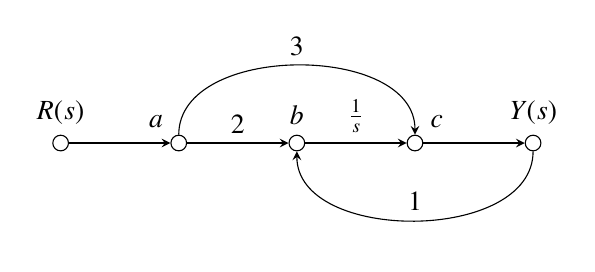
\begin{tikzpicture}[
    terminal/.style 2 args={draw,circle,inner sep=2pt,label={#1:#2}},
    amark/.style={
    ->,
    >=stealth,
    every node/.append style={above,midway}
    },
    node distance=2cm
]

%Draw the connections
\node[terminal={above}{$R(s)$}] (a) at (0,0) {};
\node[terminal={above left}{$a$}] (b) at (1.5,0) {};
\node[terminal={above}{$b$}] (c) at (3,0) {};
\node[terminal={above right}{$c$}] (d) at (4.5,0) {};
\node[terminal={above}{$Y(s)$}] (e) at (6,0) {};
%Draw the connections
\draw[amark](a) to (b);
\draw[amark] (b) to node{$2$}(c);
\draw[amark] (c) to node{$\frac{1}{s}$} (d);
\draw[amark] (b) to [bend left=90] node{$3$}(d);
\draw[amark] (d) to (e);
\draw[amark] (e) to[bend left=90] node{$1$}(c);


\end{tikzpicture}


    \caption{signal flow graph}
    \label{fig: 217.9.1.12.2}
\end{figure}
\begin{align}
    P_1 & = 2\brak{\frac{1}{s}} = \frac{2}{s}\\
    P_2 & = 3\\
    \Delta_1 & = 1 - \brak{0} = 1\\
    \Delta_2 & = 1 - \brak{0} = 1\\
    L_1 & = \frac{1}{s}\\
    \Delta & = 1 - L_1 = 1 - \frac{1}{s}
\end{align}
from \figref{fig: 217.9.1.12.2} using Mason's Gain Formula,
\begin{align}
    \frac{Y\brak{s}}{R\brak{s}} & = \frac{{\sum_{i=1}^{n} P_i\Delta_i}}{{\Delta}}\\
    & = \frac{P_1\Delta_1 + P_2\Delta_2}{\Delta}\\
    & = \frac{\frac{2}{s} + 3}{1 - \frac{1}{s}}\\
    H\brak{s} & = \frac{Y\brak{s}}{R\brak{s}} = \frac{3s+2}{s-1}
\end{align}
\begin{align}
    H\brak{s} & = \frac{5}{s-1} + 3\\
    H\brak{s} & \system{L^-1} h\brak{t}\\
    \frac{5}{s-1} & \system{L^-1} 5e^t\label{eq: 217.9.1.12.1}\\
    3 & \system{L^-1} 3\delta\brak{t}\label{eq: 217.9.1.12.2}\\
    \text{using \eqref{eq: 217.9.1.12.1} and \eqref{eq: 217.9.1.12.2},}\notag\\
    h\brak{t} & = 5e^t + 3\delta\brak{t}
\end{align}


\begin{figure}[H]
    \centering
	\includegraphics[width=\linewidth]{2023/EE/12/figs/plot.png}
    \caption{Plot of impulse response of the system}
    \label{fig: 217.9.1.12.3}
\end{figure}

\newpage

\item In the following block diagram, $R\brak{s}$ and $D\brak{s}$ are two inputs. The output Y(s) is expressed as $Y\brak{s} = G_1\brak{s}R\brak{s} + G_2\brak{s}D\brak{s}$\\
$G_1\brak{s}$ and $G_2\brak{s}$ are given by\\
\begin{figure}[htbp!]
\centering
\begin{tikzpicture}[thick,font=\large]
  \draw[-latex] (0,0) -- (2,0);
  \node at (-0.5,0) {$R\brak{s}$};
  \draw (2.5,0) circle [radius = 0.5cm];
  \node[above]  at (1.8,0) {+};
  \node[below] at (1.9,-0.3) {-};
  \draw[-latex] (3,0) -- (5,0);
  \draw (5.5,0) circle [radius=0.5cm];
  \node[above]at (4.8,0){+};
  \node[below]at (4.9,-0.3){-};
  \draw[-latex] (5.5, 2) -- (5.5,0.5);
  \node[above] at (5.5,2) {$D\brak{s}$};
  \draw[-latex] (6,0) -- (7,0);
  \draw (7,-0.5) rectangle (9, 0.5);
  \node at (8,0) {$G\brak{s}$};
  \draw[-latex] (9,0) -- (11,0);
  \node at (11.5,0) {$Y\brak{s}$};
  \draw[-] (10,0) -- (10,-3.5);
  \draw[-latex] (10,-2) -- (9,-2);
  \draw (9, -2.5) rectangle (7,-1.5);
  \node at (8,-2) {$H\brak{s}$};
  \draw[-] (7,-2) -- (5.5,-2);
  \draw[-latex] (5.5,-2) -- (5.5, -0.5);
  \draw[-] (10,-3.5) -- (2.5, -3.5);
  \draw[-latex] (2.5, -3.5) -- (2.5, -0.5);
\end{tikzpicture}

\end{figure}\\
\begin{enumerate}[label=\alph*)]
\item $G_1\brak{s} = \frac{G\brak{s}}{1+G\brak{s}+G\brak{s}H\brak{s}}$ and $G_2\brak{s} = \frac{G\brak{s}}{1+ G\brak{s}+G\brak{s}H\brak{s}}$\\
\item $G_1\brak{s} = \frac{G\brak{s}}{1+G\brak{s}+H\brak{s}}$ and $G_2\brak{s} = \frac{G\brak{s}}{1+ G\brak{s}+H\brak{s}}$\\
\item $G_1\brak{s} = \frac{G\brak{s}}{1+G\brak{s}+H\brak{s}}$ and $G_2\brak{s} = \frac{G\brak{s}}{1+ G\brak{s}+G\brak{s}H\brak{s}}$\\
\item $G_1\brak{s} = \frac{G\brak{s}}{1+G\brak{s}+G\brak{s}H\brak{s}}$ and $G_2\brak{s} = \frac{G\brak{s}}{1+ G\brak{s}+H\brak{s}}$\\
\end{enumerate}
\hfill{GATE 2023 EC Q.42}\\
\solution\\
\iffalse
\let\negmedspace\undefined
\let\negthickspace\undefined
\documentclass[journal,12pt,onecolumn]{IEEEtran}
\usepackage{cite}
\usepackage{amsmath,amssymb,amsfonts,amsthm}
\usepackage{algorithmic}
\usepackage{graphicx}
\usepackage{textcomp}
\usepackage{xcolor}
\usepackage{txfonts}
\usepackage{listings}
\usepackage{enumitem}
\usepackage{mathtools}
\usepackage{gensymb}
\usepackage{circuitikz}
\usepackage{tkz-euclide} % loads  TikZ and tkz-base
\usepackage{listings}
\usetikzlibrary{positioning,arrows,shapes}


\newtheorem{theorem}{Theorem}[section]
\newtheorem{problem}{Problem}
\newtheorem{proposition}{Proposition}[section]
\newtheorem{lemma}{Lemma}[section]
\newtheorem{corollary}[theorem]{Corollary}
\newtheorem{example}{Example}[section]
\newtheorem{definition}[problem]{Definition}
%\newtheorem{thm}{Theorem}[section] 
%\newtheorem{defn}[thm]{Definition}
%\newtheorem{algorithm}{Algorithm}[section]
%\newtheorem{cor}{Corollary}
\newcommand{\BEQA}{\begin{eqnarray}}
\newcommand{\EEQA}{\end{eqnarray}}
\newcommand{\system}[1]{\stackrel{#1}{\rightarrow}}

\newcommand{\define}{\stackrel{\triangle}{=}}
\theoremstyle{remark}
\newtheorem{rem}{Remark}
%\bibliographystyle{ieeetr}
\begin{document}
%
\providecommand{\pr}[1]{\ensuremath{\Pr\left(#1\right)}}
\providecommand{\prt}[2]{\ensuremath{p_{#1}^{\left(#2\right)} }}        % own macro for this question
\providecommand{\qfunc}[1]{\ensuremath{Q\left(#1\right)}}
\providecommand{\sbrak}[1]{\ensuremath{{}\left[#1\right]}}
\providecommand{\lsbrak}[1]{\ensuremath{{}\left[#1\right.}}
\providecommand{\rsbrak}[1]{\ensuremath{{}\left.#1\right]}}
\providecommand{\brak}[1]{\ensuremath{\left(#1\right)}}
\providecommand{\lbrak}[1]{\ensuremath{\left(#1\right.}}
\providecommand{\rbrak}[1]{\ensuremath{\left.#1\right)}}
\providecommand{\cbrak}[1]{\ensuremath{\left\{#1\right\}}}
\providecommand{\lcbrak}[1]{\ensuremath{\left\{#1\right.}}
\providecommand{\rcbrak}[1]{\ensuremath{\left.#1\right\}}}
\newcommand{\sgn}{\mathop{\mathrm{sgn}}}
\providecommand{\abs}[1]{\left\vert#1\right\vert}
\providecommand{\res}[1]{\Res\displaylimits_{#1}} 
\providecommand{\norm}[1]{\left\lVert#1\right\rVert}
%\providecommand{\norm}[1]{\lVert#1\rVert}
\providecommand{\mtx}[1]{\mathbf{#1}}
\providecommand{\mean}[1]{E\left[ #1 \right]}
\providecommand{\cond}[2]{#1\middle|#2}
\providecommand{\fourier}{\overset{\mathcal{F}}{ \rightleftharpoons}}
\newenvironment{amatrix}[1]{%
  \left(\begin{array}{@{}*{#1}{c}|c@{}}
}{%
  \end{array}\right)
}
\providecommand{\hilbert}{\overset{\mathcal{H}}{ \rightleftharpoons}}
\providecommand{\system}{\overset{\mathcal{H}}{ \longleftrightarrow}}
	%\newcommand{\solution}[2]{\textbf{Solution:}{#1}}
\newcommand{\solution}{\noindent \textbf{Solution: }}
\newcommand{\cosec}{\,\text{cosec}\,}
\providecommand{\dec}[2]{\ensuremath{\overset{#1}{\underset{#2}{\gtrless}}}}
\newcommand{\myvec}[1]{\ensuremath{\begin{pmatrix}#1\end{pmatrix}}}
\newcommand{\mydet}[1]{\ensuremath{\begin{vmatrix}#1\end{vmatrix}}}
\newcommand{\myaugvec}[2]{\ensuremath{\begin{amatrix}{#1}#2\end{amatrix}}}
\providecommand{\rank}{\text{rank}}
\providecommand{\pr}[1]{\ensuremath{\Pr\left(#1\right)}}
\providecommand{\qfunc}[1]{\ensuremath{Q\left(#1\right)}}
	\newcommand*{\permcomb}[4][0mu]{{{}^{#3}\mkern#1#2_{#4}}}
\newcommand*{\perm}[1][-3mu]{\permcomb[#1]{P}}
\newcommand*{\comb}[1][-1mu]{\permcomb[#1]{C}}
\providecommand{\qfunc}[1]{\ensuremath{Q\left(#1\right)}}
\providecommand{\gauss}[2]{\mathcal{N}\ensuremath{\left(#1,#2\right)}}
\providecommand{\diff}[2]{\ensuremath{\frac{d{#1}}{d{#2}}}}
\providecommand{\myceil}[1]{\left \lceil #1 \right \rceil }
\newcommand\figref{Fig.~\ref}
\newcommand\tabref{Table~\ref}
\newcommand{\sinc}{\,\text{sinc}\,}
\newcommand{\rect}{\,\text{rect}\,}
%%
%	%\newcommand{\solution}[2]{\textbf{Solution:}{#1}}
%\newcommand{\solution}{\noindent \textbf{Solution: }}
%\newcommand{\cosec}{\,\text{cosec}\,}
%\numberwithin{equation}{section}
%\numberwithin{equation}{subsection}
%\numberwithin{problem}{section}
%\numberwithin{definition}{section}
%\makeatletter
%\@addtoreset{figure}{problem}
%\makeatother

%\let\StandardTheFigure\thefigure
\let\vec\mathbf

\bibliographystyle{IEEEtran}





\bigskip

\renewcommand{\thefigure}{\theenumi}
\renewcommand{\thetable}{\theenumi}
%\renewcommand{\theequation}{\theenumi}


\title{GATE 2023 EC}
\author{Praful Kesavadas\\ EE23BTECH11049}
\maketitle

\textbf{Question: 42} In the following block diagram, $R\brak{s}$ and $D\brak{s}$ are two inputs. The output Y(s) is expressed as $Y\brak{s} = G_1\brak{s}R\brak{s} + G_2\brak{s}D\brak{s}$\\
$G_1\brak{s}$ and $G_2\brak{s}$ are given by\\
\begin{figure}[htbp!]
\centering
\begin{tikzpicture}[thick,font=\large]
  \draw[-latex] (0,0) -- (2,0);
  \node at (-0.5,0) {$R\brak{s}$};
  \draw (2.5,0) circle [radius = 0.5cm];
  \node[above]  at (1.8,0) {+};
  \node[below] at (1.9,-0.3) {-};
  \draw[-latex] (3,0) -- (5,0);
  \draw (5.5,0) circle [radius=0.5cm];
  \node[above]at (4.8,0){+};
  \node[below]at (4.9,-0.3){-};
  \draw[-latex] (5.5, 2) -- (5.5,0.5);
  \node[above] at (5.5,2) {$D\brak{s}$};
  \draw[-latex] (6,0) -- (7,0);
  \draw (7,-0.5) rectangle (9, 0.5);
  \node at (8,0) {$G\brak{s}$};
  \draw[-latex] (9,0) -- (11,0);
  \node at (11.5,0) {$Y\brak{s}$};
  \draw[-] (10,0) -- (10,-3.5);
  \draw[-latex] (10,-2) -- (9,-2);
  \draw (9, -2.5) rectangle (7,-1.5);
  \node at (8,-2) {$H\brak{s}$};
  \draw[-] (7,-2) -- (5.5,-2);
  \draw[-latex] (5.5,-2) -- (5.5, -0.5);
  \draw[-] (10,-3.5) -- (2.5, -3.5);
  \draw[-latex] (2.5, -3.5) -- (2.5, -0.5);
\end{tikzpicture}

\end{figure}\\
\begin{enumerate}[label=\alph*)]
\item $G_1\brak{s} = \frac{G\brak{s}}{1+G\brak{s}+G\brak{s}H\brak{s}}$ and $G_2\brak{s} = \frac{G\brak{s}}{1+ G\brak{s}+G\brak{s}H\brak{s}}$\\
\item $G_1\brak{s} = \frac{G\brak{s}}{1+G\brak{s}+H\brak{s}}$ and $G_2\brak{s} = \frac{G\brak{s}}{1+ G\brak{s}+H\brak{s}}$\\
\item $G_1\brak{s} = \frac{G\brak{s}}{1+G\brak{s}+H\brak{s}}$ and $G_2\brak{s} = \frac{G\brak{s}}{1+ G\brak{s}+G\brak{s}H\brak{s}}$\\
\item $G_1\brak{s} = \frac{G\brak{s}}{1+G\brak{s}+G\brak{s}H\brak{s}}$ and $G_2\brak{s} = \frac{G\brak{s}}{1+ G\brak{s}+H\brak{s}}$\\
\end{enumerate}
\solution\\
\fi
By superposition principle, let\\ 
\begin{align*}Y\brak{s}&= Y_1\brak{s} + Y_2\brak{s}\\ \text{where } Y_1\brak{s}&= \text{output considering only } R\brak{s}\\ Y_2\brak{s} &= \text{Output considering only } D\brak{s}
\end{align*}
When only R(s) is present:\\
\begin{figure}[ht!]
\centering
\begin{circuitikz}[scale=1.5]
    \draw
    (0,0) to[short, -*] node[pos=0] {$\textgreater$} node[pos=0.7, below=1mm] {$y_1$} node[pos=0,above=1.5mm] {$1$} (1,0) to [short, -*] node[pos=0] {$\textgreater$} node[pos=0.7,below=1mm] {$y_2$} node[pos=0, above=1.5mm] {$1$} (2,0) to [short,-*] node[pos=0]{$\textgreater$} node[pos=0,above=1mm] {$G(s)$} (3,0) to [short,-] node[pos=0, below=1mm] {$y_3$} (3.5,0);
    \draw 
    (3,0) to [out=-89,in=-89] node[pos=0.5] {$\textless$} node[pos=0.4,below=2mm] {$-H(s)$} (2,0);
    \draw (3,0) to [out=90,in=90] node[pos=0.5] {$\textless$} node[pos=0.4,above=2mm] {$-1$} (1,0);
    \node[left] at (0,0) {$R(s)$};
    \node[right] at (3.5,0) {$Y_1(s)$};
\end{circuitikz}

\end{figure}\\
By Mason's gain formula, 
\begin{align}
 \frac{Y_1\brak{s}}{R(s)} = \sum_{k=1}^n \frac{P_k.\Delta{_k}}{\Delta} \label{eq:gate.2023.ec.qn.42.1}
\end{align}
\begin{table}[ht!]
\centering
 \begin{tabular}{|c|c|}
    \hline
    \textbf{Term} & \textbf{Description}\\
    \hline
    $n$ & Number of foward paths\\
    \hline
    $\Delta{_k}$ & Associated path factor\\
    \hline
    $P_k$ & Path gain of the $k^{th}$ forward path\\
    \hline
    $\Delta$ & Determinant of Signal flow graph\\
    \hline
  \end{tabular}

\caption{Mason's Gain formula parameters}
\end{table}\\
Here, 
\begin{align}
 n&=1\brak{\text{i.e path } R-y_1-y_2-y_3-Y_1}\\
 P_1&= G\brak{s}\\
 \Delta{_1}&= 1 \brak{\text{As no isolated node is present}}\\
 \Delta &= 1+ G\brak{s} + G\brak{s}H\brak{s}
\end{align}
Substituting in \eqref{eq:gate.2023.ec.qn.42.1},
\begin{align}
\frac{Y_1\brak{s}}{R\brak{s}} &= \frac{G\brak{s}}{1+G\brak{s} + G\brak{s}H\brak{s}}\\
Y_1\brak{s} &= \sbrak{\frac{G\brak{s}}{1+ G\brak{s}+ G\brak{s}H\brak{s}}} R\brak{s}
\end{align}
Hence,
\begin{align}
 G_1\brak{s} = \frac{G\brak{s}}{1+G\brak{s}+G\brak{s}H\brak{s}}
\end{align}
When only $D\brak{s}$ is present:
\begin{figure}[ht!]
\centering
\begin{circuitikz}[scale=1.5]
    \draw
    (0,0) to[short, -*] node[pos=0] {$\textgreater$} node[pos=0.7, below=1mm] {$y_1$} node[pos=0,above=1.5mm] {$1$} (1,0) to [short,-*] node[pos=0] {$\textgreater$} node[pos=0,above=2mm] {$G(s)$} (3,0) to [short,-] node[pos=0,below=1mm] {$y_2$} (3.5,0);
    
    \draw (3,0) to [out=-90,in=-90] node[pos=0.5] {$\textless$} node[pos=0.4,below=2mm] {$-1$} (1,0);
    \draw (3,0) to [out=90,in=90] node[pos=0.5] {$\textless$} node[pos=0.4,above=2mm] {$-H(s)$} (1,0);
    \node[left] at (0,0) {$D(s)$};
    \node[right] at (3.5,0) {$Y_2(s)$};
\end{circuitikz}

\end{figure}\\
Here, 
\begin{align}
 n&=1\brak{\text{i.e path } D-y_1-y_2-Y_2}\\
 P_1&= G\brak{s}\\
 \Delta{_1}&= 1 \\
 \Delta &= 1+ G\brak{s} + G\brak{s}H\brak{s}
\end{align}
Substituting in \eqref{eq:gate.2023.ec.qn.42.1},
\begin{align}
\frac{Y_2\brak{s}}{D\brak{s}}&= \frac{G\brak{s}}{1+ G\brak{s}+G\brak{s}H\brak{s}}\\
Y_2\brak{s}&= \sbrak{\frac{G\brak{s}}{1+ G\brak{s}+ G\brak{s}H\brak{s}}} D\brak{s}
\end{align}
Hence,
\begin{align}
G_2\brak{s} &= \frac{G\brak{s}}{1+ G\brak{s}+ G\brak{s}H\brak{s}}
\end{align}
Option \brak{a} is correct
%\end{document}

\newpage

\item In the table shown below, match the signal type with its spectral characteristics.\hfill{GATE 2023 EC}

\vspace{2mm}

\begin{table}[ht]
    \centering
    \def\arraystretch{2.5}
    \begin{tabular}{|c|c|}
\hline
Signal Type & Spectral Characterstics \\
\hline
$\brak{i}$  Continuous, aperiodic & \brak{a} Continuous, aperiodic\\
\hline
$\brak{ii}$ Continuous, periodic & \brak{b} Continuous, periodic \\
\hline
$\brak{iii}$ Discrete, aperiodic & \brak{c} Discrete, aperiodic\\
\hline
$\brak{iii}$ Discrete, periodic & \brak{d} Discrete, periodic\\
\hline
\end{tabular}
    \caption{ }
    \label{29.2023}
\end{table}

\begin{enumerate}
\item \brak{\romannumeral 1} \textrightarrow \brak{a}  ,   \brak{\romannumeral 2} \textrightarrow \brak{b}   ,   \brak{\romannumeral 3} \textrightarrow \brak{c}   ,   \brak{\romannumeral 4} \textrightarrow \brak{d}

\item \brak{\romannumeral 1} \textrightarrow \brak{a}   ,  \brak{\romannumeral 2} \textrightarrow \brak{c}   ,   \brak{\romannumeral 3} \textrightarrow \brak{b}   ,   \brak{\romannumeral 4} \textrightarrow \brak{d}

\item  \brak{\romannumeral 1} \textrightarrow \brak{d}   ,   \brak{\romannumeral 2} \textrightarrow \brak{b}   ,   \brak{\romannumeral 3} \textrightarrow \brak{c}   ,   \brak{\romannumeral 4} \textrightarrow \brak{a}

\item \brak{\romannumeral 1} \textrightarrow \brak{a}   ,  \brak{\romannumeral 2} \textrightarrow \brak{c}    ,   \brak{\romannumeral 3} \textrightarrow \brak{d}   ,  \brak{\romannumeral 4} \textrightarrow \brak{b}

\end{enumerate}
\solution
\iffalse
\let\negmedspace\undefined
\let\negthickspace\undefined
\documentclass[journal,12pt,onecolumn]{IEEEtran}
\usepackage{cite}
\usepackage{amsmath,amssymb,amsfonts,amsthm}
\usepackage{algorithmic}
\usepackage{graphicx}
\usepackage{textcomp}
\usepackage{xcolor}
\usepackage{txfonts}
\usepackage{listings}
\usepackage{enumitem}
\usepackage{mathtools}
\usepackage{gensymb}
\usepackage{comment}
\usepackage[breaklinks=true]{hyperref}
\usepackage{tkz-euclide} 
\usepackage{listings}
\usepackage{gvv}                                        
\def\inputGnumericTable{}                                 
\usepackage[latin1]{inputenc}                                
\usepackage{color}                                            
\usepackage{array}                                            
\usepackage{longtable}                                       
\usepackage{calc}                                             
\usepackage{multirow}                                         
\usepackage{hhline}                                           
\usepackage{ifthen}                                           
\usepackage{lscape}
\usepackage{textcomp}

\newtheorem{theorem}{Theorem}[section]
\newtheorem{problem}{Problem}
\newtheorem{proposition}{Proposition}[section]
\newtheorem{lemma}{Lemma}[section]
\newtheorem{corollary}[theorem]{Corollary}
\newtheorem{example}{Example}[section]
\newtheorem{definition}[problem]{Definition}
\newcommand{\BEQA}{\begin{eqnarray}}
\newcommand{\EEQA}{\end{eqnarray}}
\newcommand{\define}{\stackrel{\triangle}{=}}
\theoremstyle{remark}
\newtheorem{rem}{Remark}
\begin{document}

\bibliographystyle{IEEEtran}
\vspace{3cm}

\title{ec23...}
\author{EE23BTECH11029 - Kanishk}
\maketitle

\bigskip

\renewcommand{\thefigure}{\theenumi}
\renewcommand{\thetable}{\theenumi}
\textbf{Question}:\\ 
In the table shown below, match the signal type with its spectral characteristics.\hfill{GATE 2023 EC}

\vspace{2mm}

\begin{table}[ht]
    \centering
    \def\arraystretch{2}
    \begin{tabular}{|c|c|}
\hline
Signal Type & Spectral Characterstics \\
\hline
$\brak{i}$  Continuous, aperiodic & \brak{a} Continuous, aperiodic\\
\hline
$\brak{ii}$ Continuous, periodic & \brak{b} Continuous, periodic \\
\hline
$\brak{iii}$ Discrete, aperiodic & \brak{c} Discrete, aperiodic\\
\hline
$\brak{iii}$ Discrete, periodic & \brak{d} Discrete, periodic\\
\hline
\end{tabular}
    \caption{ }
    \label{29.2023}
\end{table}

\begin{enumerate}
\item \brak{\romannumeral 1} \textrightarrow \brak{a}  ,   \brak{\romannumeral 2} \textrightarrow \brak{b}   ,   \brak{\romannumeral 3} \textrightarrow \brak{c}   ,   \brak{\romannumeral 4} \textrightarrow \brak{d}

\item \brak{\romannumeral 1} \textrightarrow \brak{a}   ,  \brak{\romannumeral 2} \textrightarrow \brak{c}   ,   \brak{\romannumeral 3} \textrightarrow \brak{b}   ,   \brak{\romannumeral 4} \textrightarrow \brak{d}

\item  \brak{\romannumeral 1} \textrightarrow \brak{d}   ,   \brak{\romannumeral 2} \textrightarrow \brak{b}   ,   \brak{\romannumeral 3} \textrightarrow \brak{c}   ,   \brak{\romannumeral 4} \textrightarrow \brak{a}

\item \brak{\romannumeral 1} \textrightarrow \brak{a}   ,  \brak{\romannumeral 2} \textrightarrow \brak{c}    ,   \brak{\romannumeral 3} \textrightarrow \brak{d}   ,  \brak{\romannumeral 4} \textrightarrow \brak{b}

\end{enumerate}

\textbf{Solution}:\\
\fi


\begin{table}[ht]
    \centering
    \def\arraystretch{2}
    \begin{tabular}{|c|c|}
\hline
Parameter & Description \\
\hline
$x\brak{t}$  & Continuous Time  Signal\\
\hline
$x\brak{f}$ & Fourier Transform of a Signal \\
\hline
$x\sbrak{n}$ & Discrete Time Signal\\
\hline
$X\sbrak{k}$ &  Tthe amplitude and phase of the $k^{th}$frequency component of the input signal $x\sbrak{n}$\\
\hline
$u\brak{t}= \begin{cases}  0 & t<0\\ 1 & t\geq0 \end{cases}$ & Unit step signal in continuous time\\
\hline
$u\sbrak{n}= \begin{cases}  0 & n<0\\ 1 & n\geq0 \end{cases}$ & Unit step signal Discrete time \\
\hline
$x\brak{t}= e^{-2t}.u\brak{t}$ & Exponential Decay Continuous time Signal\\
\hline
$x\brak{t}=sin\brak{2\pi ft}$ & Sine wave Continuous time Signal\\
\hline
$x\sbrak{n}=e^{n}.u\sbrak{n} $& Exponential Decay Discrete time Signal\\
\hline
$x\sbrak{n}= sin\brak{2\pi f_0 n}.u\sbrak{n}$ & Sinusoidal Discrete time Signal\\
\hline
\end{tabular}
    \caption{Input Parameters}
    \label{tab:gate_2023_ec29}
\end{table}

\newpage
\textbf{1. Continuous, aperiodic signal}\\

\begin{align}
X\brak{f}&=\int_{-\infty}^{\infty} x\brak{t}.e^{-j2\pi ft}\,dt
\end{align}

Let's consider the limit as $f$ approaches a certain frequency $f_0$:

\begin{align}
lim_{\epsilon \rightarrow 0}X\brak{f_0+\epsilon}&= lim_{\epsilon \rightarrow 0}\int_{-\infty}^{\infty} x\brak{t}.e^{-j2\pi ft}\,dt
\end{align}

By continuity of $x\brak{t}$ we can interchange the limit and the integral:
\begin{align}
&=\int_{-\infty}^{\infty} x\brak{t}.lim_{\epsilon\rightarrow0}e^{-j2\pi\brak{f_0+\epsilon}t}\,dt\\
&=\int_{-\infty}^{\infty} x\brak{t}.e^{-j2\pi f_0 t}\,dt\\
&=X\brak{f_0}\\
 lim_{f_0-\epsilon}&=X\brak{f_0}
\end{align}

Therefore, X\brak{f} is continuous for all frequencies $f$.

Let's assume $X\brak{f}$ is periodic with period $T$ 

\begin{align}
X\brak{f+T}&=X\brak{f}
\end{align}
Now applying inverse Fourier transform

\begin{align}
x\brak{t}&=\int_{-\infty}^{\infty} X\brak{f}.e^{j2\pi ft}\,df\\
&=\int_{-\infty}^{\infty} X\brak{f+T}.e^{j2\pi \brak{f+T}t}\,df\\
&=\int_{-\infty}^{\infty} X\brak{f}.e^{j2\pi \brak{f+T}t}\,df\\
&=e^{j2\pi Tt}\int_{-\infty}^{\infty}.X\brak{f}.e^{2\pi ft}\, df
\end{align}

$e^{j2\pi Tt}$ is a periodic function of $t$, which contradicts that $x\brak{t}$ is aperiodic,

Therefore, $X\brak{f}$ cannot be periodic, hence it must be aperiodic.\\
\vspace{2mm}


For Example: Exponential Decay\\

From \tabref{tab:gate_2023_ec29}
\begin{align}
x\brak{t}&=e^{-2 t}.u\brak{t}\\
X\brak{f}&= \int_{-\infty}^{\infty} e^{-2ft}u\brak{t}.e^{-j2\pi ft}\,dt\\
&= \int_{0}^{\infty} e^{-\brak{2+j2\pi f}t}\,dt\\
&= \frac{1}{2\brak{1 + j\pi f}}
\end{align}

$\implies X\brak{f} $ is continuous and aperiodic \\
 

\textbf{2. Continuous, periodic signal}\\

\begin{align}
x\brak{t}&=x\brak{t+kT}\\
x\brak{t}& \leftrightarrow X\brak{f}\\
X\brak{f}&=\int_{-\infty}^{\infty} x\brak{t}.e^{-j2\pi ft}\,dt\\
X\brak{f}&=\int_{-\infty}^{\infty} x\brak{t+kT}.e^{-j2\pi ft}\,dt\\
\text{Let } \tau &= t+kT\\
X\brak{f}&=\int_{-\infty}^{\infty} x\brak{\tau}.e^{-j2\pi f\tau}.e^{j2\pi fkT}\,d\tau
\end{align}

$e^{j2\pi fkT} $ is a Periodic function in frequency domain with period $\frac{1}{T}$ Hz \\
\begin{align}
X\brak{f}&=e^{j2\pi fkT}\int_{-\infty}^{\infty} x\brak{\tau}.e^{-j2\pi f\tau}\,d\tau\\
\implies &X\brak{f} \text{ is aperiodic}
\end{align}


$X\brak{f}$ will be  a sum of scaled copies of the Fourier transform of $x\brak{t}$, each copy shifted by multiples of $\frac{1}{T}$Hz This results in a discrete frequency domain representation.\\
\vspace{2mm}

For example: Sine wave function\\

From \tabref{tab:gate_2023_ec29}
\begin{align}
x\brak{t}&=sin\brak{2\pi ft}\\
sin\brak{f_0t}&= \frac{1}{2j}\sbrak{e^{j2\pi f_0 t} -  e^{-j2\pi f_0 t} }\\
X\brak{f} &=  \frac{1}{2j}  \sbrak{2\pi \delta\brak{2\pi f- 2\pi f_0} - 2\pi \delta\brak{2\pi f+2\pi f_0}  }\\
&= j\pi \sbrak{\delta\brak{2\pi f + 2\pi f_0} -   \delta\brak{2\pi f - 2\pi f_0}}
\end{align}

$\implies X\brak{f}$ is Discrete and Aperiodic Signal\\


\textbf{3. Discrete, aperiodic signal}\\

\begin{align}
X\brak{e^{j2\pi f}}&= \sum_{n=-\infty}^{\infty} x\sbrak{n}.e^{-j2\pi fn}
\end{align}


Let's consider the Discrete time Fourier Transform (DFT) of $x\sbrak{n}$, denoted by $ X\sbrak{k}$ which is defined as:

\begin{align}
X\sbrak{k}&=\sum_{n=0}^{N-1}x\sbrak{n}e^{-j\frac{2\pi}{N}kn}
\end{align}
The DFT is inherently periodic in frequency domain with period $\frac{1}{N}$.\\


As  $N$ approaches infinity, the spacing between frequency samples in the frequency domain  $\frac{1}{N}$  approaches zero. Therefore, the DFT $X\sbrak{k}$ approaches the continuous Fourier Transform $X\brak{f}$. \\

Since the DFT $X\brak{f}$  is periodic in the frequency domain, its limiting form $X\brak{f}$ is also periodic, continuous in frequency domain.\\

For example: Exponential Decay\\

From \tabref{tab:gate_2023_ec29}

\begin{align}
x\sbrak{n}&= e^{n}.u\sbrak{n}\\
X\brak{e^{j2\pi f}}&= \sum_{n=-\infty}^{\infty} e^{n}.u\sbrak{n}.e^{-j2\pi fn}\\
&=  \sum_{n=0}^{\infty} e^{\brak{1-j2\pi f}^{n}}\\
&=\frac{1}{1-e^{\brak{1-j2\pi f}}}
\end{align}
$\implies $ Continuous and Periodic signal\\

\vspace{2mm}
\textbf{4. Discrete,periodic signal}

\begin{align}
X\brak{f}&= \sum_{n=-\infty}^{\infty} x\sbrak{n}.e^{-j2\pi fn}
\end{align}

The Discrete Fourier Transform(DFT) is periodic in frequency domain with period $\frac{1}{N}$\\

As $N$ is finite , Therefore DFT has finite period $\frac{1}{N}$

\begin{align}
X\sbrak{k}&=\sum_{n=0}^{N-1}x\sbrak{n}e^{-j\frac{2\pi}{N}kn}
\end{align}
The DFT computation involves summing over a finite number of samples . Therefore, the resulting spectrum  $X\sbrak{k}$ is inherently discrete.\\

For example:  Sinusoidal Signal\\

From \tabref{tab:gate_2023_ec29}

\begin{align}
x\sbrak{n}&=sin\brak{2\pi f_0n}.u\sbrak{n}\\
X\brak{e^{j2\pi f}}&= \sum_{n=-\infty}^{\infty} sin\brak{2\pi f_0n}.u\sbrak{n}.e^{-j2\pi fn}\\
&= \sum_{n=0}^{\infty} \frac{e^{j2\pi f_0n}- e^{-j2\pi f_0n}}{2j}. e^{-j2\pi fn}\\
&=\frac{1}{2j}\sum_{n=0}^{\infty} \brak{e^{j\brak{2\pi f_0n-2\pi fn}} -  e^{-j\brak{2\pi f_0n+2\pi fn}} }\\
&= \frac{1}{2j} \brak{\frac{1}{1-e^{j\brak{2\pi f_0-2\pi f}}}  -  \frac{1}{1-e^{-j\brak{2\pi f_0+ 2\pi f}}}}
\end{align}
$\implies$Discrete and Periodic \\

\brak{\romannumeral 1} \textrightarrow \brak{a}   ,  \brak{\romannumeral 2} \textrightarrow \brak{c}   ,   \brak{\romannumeral 3} \textrightarrow \brak{b}   ,   \brak{\romannumeral 4} \textrightarrow \brak{d}

%\end{document}

\newpage


\item
The impulse response of an LTI system is $h\brak{t}$= $\delta\brak{t}$+0.5$ \delta\brak{t-4}$, where $\delta\brak{t}$ is continuous-time unit impulse signal.If the input signal $x(t)=\cos\brak{\frac{7\pi t}{4}}$,the output is\hfill(GATE IN 2023)\\
\solution 
\iffalse
\documentclass[journal,12pt,twocolumn]{IEEEtran}
\usepackage{amsmath,amssymb,amsfonts,amsthm}
\usepackage{txfonts}
\usepackage{tkz-euclide}
\usepackage{listings}
\usepackage{gvv}
\usepackage[latin1]{inputenc}
\usepackage{array}
\usepackage{pgf}
\usepackage{lmodern}

\begin{document}
\bibliographystyle{IEEEtran}

\title{GATE 2023[IN]-36}
\author{EE23BTECH11066 - Yakkala Amarnath Karthik}
\maketitle
\bibliographystyle{IEEEtran}
\textbf{Question:}\\ \\
The impulse response of an LTI system is $h\brak{t}$= $\delta\brak{t}$+0.5$ \delta\brak{t-4}$, where $\delta\brak{t}$ is continuous-time unit impulse signal.if the input signal $x(t)=\cos\brak{\frac{7\pi t}{4}}$,the output is\hfill(GATE IN 2023)\\ \\

\textbf{Solution:}\\
\fi
\begin{table}[ht]
  \begin{tabular}{|c|c|c|}
    \hline
    \textbf{Variable} & \textbf{Description} & \textbf{value}\\
    \hline
    $\delta\brak{t}$ & Dirac delta function &$\infty$ if t=0;  0 in other cases \\& &$\int_{-\infty} ^ {\infty} \delta\brak{t}=1$\\
   \hline
    $h\brak{t}$ & impulse response & $\delta\brak{t}$+0.5$ \delta\brak{t-4}$ \\
    \hline
    $x\brak{t}$ & input signal  & $x(t)=cos\brak{\frac{7\pi t}{4}}$ \\
    \hline
$y\brak{t}$ & output signal & x\brak{t}$ *$ h\brak{t} \\
    \hline
     $\mathcal{F}\brak{\cos{a t}}$ & Fourier transform of $\cos{a t}$ & $0.5\sbrak{\delta \brak{f-\frac{a}{2\pi}}+\delta \brak{f+\frac{a}{2\pi}}}$\\
    \hline
    $X\brak{f}$ & Fourier transform of $x\brak{t}$ & $0.5\sbrak{\delta \brak{f-\frac{7}{8}}+\delta \brak{f+\frac{7}{8}}}$\\
    \hline
        $H\brak{f}$ & Fourier transform of $h\brak{t}$ & 1+0.5$e^{-j8\pi f}$\\
    \hline
     $Y\brak{f}$ & Fourier transform of $y\brak{t}$ & $X\brak{f}H\brak{f}$\\
    \hline
    \end{tabular}
  \caption{A Table with input parameters}
  \label{tab:gate2023in36}
\end{table}
\\
 from \tabref{tab:gate2023in36}
\begin{align}
    y\brak{t} &=x\brak{t} * h\brak{t}\\
            &=x\brak{t} * \brak{\delta\brak{t}+0.5 \delta\brak{t-4}}\\
            &=x\brak{t}+0.5x\brak{t-4}\\
            &=\cos\brak{\frac{7\pi t}{4}}+0.5\cos\brak{\frac{7\pi \brak{t-4}}{4}}\\
            &=\cos\brak{\frac{7\pi t}{4}}+0.5\cos\brak{\frac{7\pi t}{4}-7\pi}\\
            &=\frac{1}{2}\cos\brak{\frac{7\pi t}{4}}\\
            &=\frac{1}{2}x\brak{t}
\end{align}

\begin{align}
    Y\brak{f} &= X\brak{f}H\brak{f}\\
   &=\frac{1}{2}\sbrak{\delta \brak{f-\frac{7}{8}}+\delta \brak{f+\frac{7}{8}}}\sbrak{1+0.5e^{-j8\pi f}}
         \end{align} \\ \\
 \vspace{7.2cm}
\begin{align}
  \hspace{1.2cm}Y\brak{f} &=\frac{1}{2}\brak{1+0.5e^{-j8\pi f}}\delta \brak{f-\frac{7}{8}}+\nonumber\\
   &\frac{1}{2}\brak{1+0.5e^{-j8\pi f}}\delta \brak{f+\frac{7}{8}}\\
   &=\frac{1}{2}\brak{1+0.5\brak{-1}}\delta \brak{f-\frac{7}{8}}+\nonumber\\
   &\frac{1}{2}\brak{1+0.5\brak{-1}}\delta \brak{f+\frac{7}{8}}\\
  &=\frac{1}{4}\sbrak{\delta \brak{f-\frac{7}{8}}+\delta \brak{f+\frac{7}{8}}}\\
   &=\frac{1}{2}X\brak{f}
\end{align}

\begin{figure}[ht]
    \centering
    \includegraphics[width=0.45\textwidth]{2023/IN/36/figs/pythongate.png}
    \caption{Graph showing x(t) and y(t)}
\end{figure}


\newpage

\newpage

\item Consider the state-space description of an LTI system with matrices
\[ 
A = \begin{bmatrix} 0 & 1 \\ -1 & -2 \end{bmatrix}, \quad 
B = \begin{bmatrix} 0 \\ 1 \end{bmatrix}, \quad 
C = \begin{bmatrix} 3 & -2 \end{bmatrix}, \quad 
D = 1 
\]

For the input, $\sin(\omega t)$, $\omega > 0$, the value of $\omega$ for which the steady-state output of the system will be zero, is \underline{\hspace{2cm}} (Round off to the nearest integer).
\hfill(GATE 2023 EE Q46)\\
\solution
\input{2023/EE/46/gate46.tex}
\newpage

\item A causal, discrete time system is described by the difference equation $y[n] = 0.5 y[n-1] + x[n]$, for all $n$, where $y[n]$ denotes the output sequence and $x[n]$ denotes the input sequence. Which of the following statements is/are TRUE?

\begin{enumerate}[label = (\alph*)]
	\item he system has an impulse response described by $0.5^{n} u[-n]$ where $u[n]$ is the  
unit step sequence. 		
	\item The system is stable in the bounded input, bounded output sense.
	\item The system has an infinite number of non-zero samples in its impulse response
	\item The system has a finite number of non-zero samples in its impulse response.
\end{enumerate}

\hfill(GATE 2023 BM-26)\\
\solution
\iffalse
\let\negmedspace\undefined
\let\negthickspace\undefined
\documentclass[journal,12pt,twocolumn]{IEEEtran}
\usepackage{cite}
\usepackage{amsmath,amssymb,amsfonts}
\usepackage{graphicx}
\usepackage{textcomp}
\usepackage{xcolor}
\usepackage{txfonts}
\usepackage{listings}
\usepackage{enumitem}
\usepackage{mathtools}
\usepackage{gensymb}
\usepackage{comment}
\usepackage[breaklinks=true]{hyperref}
\usepackage{tkz-euclide} 
\usepackage{listings}
\usepackage{gvv}                                        
\def\inputGnumericTable{}                                 
\usepackage[latin1]{inputenc}                                
\usepackage{color}                                            
\usepackage{array}                                            
\usepackage{longtable}                                       
\usepackage{calc}                                             
\usepackage{multirow}                                         
\usepackage{hhline}                                           
\usepackage{ifthen}                                           
\usepackage{lscape}
\usepackage[export]{adjustbox}

\newtheorem{theorem}{Theorem}[section]
\newtheorem{problem}{Problem}
\newtheorem{proposition}{Proposition}[section]
\newtheorem{lemma}{Lemma}[section]
\newtheorem{corollary}[theorem]{Corollary}
\newtheorem{example}{Example}[section]
\newtheorem{definition}[problem]{Definition}
\newcommand{\BEQA}{\begin{eqnarray}}
\newcommand{\EEQA}{\end{eqnarray}}
\newcommand{\define}{\stackrel{\triangle}{=}}
\newtheorem{rem}{Remark}

\begin{document}
\parindent 0px
\bibliographystyle{IEEEtran}

\vspace{3cm}

\title{}
\author{EE23BTECH11042 -  Khusinadha Naik$^{*}$
}
\maketitle
\newpage
\bigskip

% \renewcommand{\thefigure}{\theenumi}
% \renewcommand{\thetable}{\theenumi}


\noindent \textbf{26.} \hspace{2pt}A casual, discrete time system is described by the difference equation $y[n] = 0.5 y[n-1] + x[n]$, for all $n$, where $y[n]$ denotes the output sequence and $x[n]$ denotes the input sequence. Which of the following statements is/are TRUE?
\begin{flushright}
\hfill(GATE 2023 BM)
\end{flushright}
\begin{enumerate}[label = (\alph*)]
	\item The system has an impulse response described by $0.5^{n} u[-n]$ where $u[n]$ is the  
unit step sequence. 		
	\item The system is stable in the bounded input, bounded output sense.		
	\item The system has an infinite number of non-zero samples in its impulse response	
	\item The system has a finite number of non-zero samples in its impulse response.
\end{enumerate}

\noindent \textbf{Ans.}\\
\fi
\begin{table}[h]
\centering
\begin{tabular}{|c|c|c|}
        \hline
        \textbf{Parameter} & \textbf{Value} & \textbf{Description} \\
        \hline
        $x[n]$ & ? & Input Sequence \\
        \hline
        $y[n]$ & ? & Output Sequence \\
        \hline
\end{tabular}
\caption{Input parameters table}
\label{tab:GATE.2023.BM.26.1}





\end{table}
\begin{align}
y[n] = 0.5y[n-1] + x[n] 
\end{align}

Taking $Z$-Transform 
\begin{align}
Y\brak{z} &= 0.5z^{-1}Y\brak{z} + X\brak{z} \\
\implies \frac{Y\brak{z}}{X\brak{z}} &= \frac{1}{1 - 0.5z^{-1}} = H\brak{z} 
\end{align}
If $x[n]$ is impulse input 
\begin{align}
\implies &Y\brak{z} = H\brak{z} = \frac{1}{1 - 0.5z^{-1}}  \label{eq:GATE.2023.BM.26.4}
\end{align}
From \eqref{eq:GATE.2023.BM.26.4} pole lies at $z = 0.5$
\begin{align}
a^{n}u\brak{n} \xleftrightarrow{\mathcal{Z}} &\frac{1}{1 - az^{-1}} \quad , \abs{z} > a \label{eq:GATE.2023.BM.26.5}
\end{align}

From \eqref{eq:GATE.2023.BM.26.4} , \eqref{eq:GATE.2023.BM.26.5}
\begin{align}
h[n] = 0.5^{n}u[n] \quad , \abs{z} > 0.5 \label{eq:GATE.2023.BM.26.6}
\end{align}
\pagebreak 
Plotting $h[n]$ vs $n$
\begin{figure}[h]
    \includegraphics[width=0.5\textwidth]{2023/BM/26/figs/fig1.png}
    \caption{Plot of $h[n]$ vs $n$}
    \label{fig:GATE.2023.BM.26.1}
\end{figure}

\begin{enumerate}
\item From \eqref{eq:GATE.2023.BM.26.6} , (a) is wrong
\item As pole lies within unit circle (b) is true
\item From \eqref{eq:GATE.2023.BM.26.6} and \figref{fig:GATE.2023.BM.26.1} ,(c) is true and hence
\item (d) is false 
\end{enumerate}





%\end{document}

\newpage

\item A closed loop system is shown in the figure where $k>0$ and $\alpha>0$. The steady state
error due to a ramp input $\brak{R\brak{s} = \alpha s^{-2}}$  is given by \hfill{(GATE 2023 EC 41)}

\begin{figure}[ht]
\centering
    \includegraphics[width=1.0\linewidth]{2023/EC/41/figs/question.png}
\end{figure}
\begin{enumerate}[label = (\alph*)]
  \item $\frac{2\alpha}{k}$    
  \item $\frac{\alpha}{k}$
  \item $\frac{\alpha}{2k}$
  \item $\frac{\alpha}{4k}$
\end{enumerate}
    
\solution
\iffalse
\let\negmedspace\undefined
\let\negthickspace\undefined
\documentclass[journal,12pt,twocolumn]{IEEEtran}
\usepackage{cite}
\usepackage{amsmath,amssymb,amsfonts,amsthm}
\usepackage{algorithmic}
\usepackage{graphicx}
\usepackage{textcomp}
\usepackage{xcolor}
\usepackage{txfonts}
\usepackage{listings}
\usepackage{enumitem}
\usepackage{mathtools}
\usepackage{gensymb}
\usepackage{comment}
\usepackage[breaklinks=true]{adjustbox}
\usepackage{tkz-euclide} 
\usepackage{listings}
\usepackage{gvv}                                        
\def\inputGnumericTable{}                                 
\usepackage[latin1]{inputenc}                                
\usepackage{color}                                            
\usepackage{array}                                            
\usepackage{longtable}                                       
\usepackage{calc}                                             
\usepackage{multirow}                                         
\usepackage{hhline}                                           
\usepackage{ifthen}                                           
\usepackage{lscape}

\newtheorem{theorem}{Theorem}[section]
\newtheorem{problem}{Problem}
\newtheorem{proposition}{Proposition}[section]
\newtheorem{lemma}{Lemma}[section]
\newtheorem{corollary}[theorem]{Corollary}
\newtheorem{example}{Example}[section]
\newtheorem{definition}[problem]{Definition}
\newcommand{\BEQA}{\begin{eqnarray}}
\newcommand{\EEQA}{\end{eqnarray}}
\newcommand{\define}{\stackrel{\triangle}{=}}
\theoremstyle{remark}
\newtheorem{rem}{Remark}

\begin{document}
\bibliographystyle{IEEEtran}

\vspace{3cm}

\title{}
\author{EE23BTECH11024 - G.Karthik Yadav$^{*}$
}
\maketitle
\newpage
\bigskip

\section*{GATE 2023 EC 41}
\noindent 1. \hspace{2pt} A Closed loop systen is shown in the figure where $k>0$ and $\alpha>0$ .\\
The Steady State error due to a ramp input $\brak{R\brak{s} = \alpha s^{-2}}$ is given by \hfill{(GATE 2023 EC 41)}

\begin{figure}[ht]
\centering
    \includegraphics[width=1.0\linewidth]{2023/EC/41/figs/question.png}
    \label{fig: 23.EC.41.24.1}
\end{figure}

\begin{enumerate}
\item $\frac{2\alpha}{k}$
\item $\frac{\alpha}{k}$
\item $\frac{\alpha}{2k}$
\item $\frac{\alpha}{4k}$
\end{enumerate}

\solution\\
\fi
\begin{table}[ht]
\setlength{\arrayrulewidth}{0.3mm}
\setlength{\tabcolsep}{15pt}
\renewcommand{\arraystretch}{1.5}



\begin{tabular}{ |p{1cm}|p{3cm}|p{1cm}| }
\hline
Symbol & Parameters & Value\\
\hline
$R\brak{s}$ & Laplace transform Ramp input signal r\brak{t} &  $\alpha s^{-2}$\\
\hline
$G\brak{s}$ & Open Loop transfer function &  $ \frac{Y\brak{s}}{E\brak{s}} = \frac{k}{s\brak{s+2}}$\\
\hline
$Y\brak{s}$ & Laplace transform of the output signal y\brak{t}  &  ? \\
\hline
$E\brak{s}$ & Laplace transform of the error signal e\brak{t} & R\brak{s} - Y\brak{s}\\
\hline
$E\brak{s}$ & Laplace transform of the error signal e\brak{t} & R\brak{s} - Y\brak{s}\\   
\hline
$e_s$ & Steady State Error &  ? \\
\hline
%$x(l)$ & Last($l^{th}$) term of series & 350\\
%$x(0)$ & Starting ($0^{th}$) term of series & 17 %\\
%\hline
%d & Common difference of AP & 9\\
%\hline
\end{tabular}
\caption{Parameters}






\end{table}
\bigskip
from table  Open loop transfer function $G\brak{s}$\\
\begin{align}
	G\brak{s} &= \frac{Y\brak{s}}{E\brak{s}} \label{24.2023.EC.41.1} \\
        &= \frac{Y\brak{s}}{R\brak{s} - Y\brak{s}} \\
        Y\brak{s} &= \frac{R\brak{s}G\brak{s}}{1 + G\brak{s}} \label{24.2023.EC.41.2}
\end{align}

from eq \ref{24.2023.EC.41.1} and eq \eqref{24.2023.EC.41.2}

\begin{align}
        G\brak{s} &= \frac{k}{s\brak{s +2}}  \label{24.2023.EC.41.3} \\ 
        Y\brak{s} &= \frac{\alpha k s^{-2}}{k + s\brak{s+2}} \label{24.2023.EC.41.4} \\
        E\brak{s} &= R\brak{s} - Y\brak{s}  \label{24.2023.EC.41.5} \\ 
        E\brak{s} &= \frac{\alpha \brak{s+2}}{s\brak{k + s\brak{s+2}}}
\end{align}

By Taking Inverse Laplace Transform of eq \eqref{24.2023.EC.41.3} and eq\eqref{24.2023.EC.41.4}

\begin{align}
    g\brak{t} &= \frac{k\brak{1 - e^{-2t}}}{2} u\brak{t} \\
        y\brak{t} &= \alpha t u\brak{t}- \frac{2\alpha}{k}u\brak{t} \\
        \notag &+\frac{\alpha}{2k\sqrt{1-k}} \biggl(2\sqrt{1-k}e^{\sqrt{1-k}t-1}\\ 
        \notag &+ 2\sqrt{1-k}e^{-\sqrt{1-k}t-1} \\
        \notag &+ \brak{2-k}e^{\sqrt{1-k}t-1} - \brak{2-k}e^{-\sqrt{1-k}t-1} \biggr) u\brak{t}
\end{align}

\begin{align}
        e\brak{t} &= r\brak{t} - y\brak{t} \\
        &= \alpha t u\brak{t} - y\brak{t} \\
        e\brak{t} &= \frac{2\alpha}{k}u\brak{t} \\
        \notag &-\frac{\alpha}{2k\sqrt{1-k}} \biggl(2\sqrt{1-k}e^{\sqrt{1-k}t-1}\\ 
        \notag &+ 2\sqrt{1-k}e^{-\sqrt{1-k}t-1} \\
        \notag &+ \brak{2-k}e^{\sqrt{1-k}t-1} - \brak{2-k}e^{-\sqrt{1-k}t-1} \biggr) u\brak{t}
\end{align}
	

\begin{align}
    e_s &= \displaystyle\lim_{s\to 0}s E\brak{s} \\
    &= \displaystyle\lim_{s\to 0} s \frac{R\brak{s}}{1 + G\brak{s}} \\
    &= \displaystyle\lim_{s\to 0} \frac{\alpha \brak{s+2}}{s\brak{s+2} + k} \\
    e_s &= \frac{2\alpha}{k}
\end{align}



\newpage

\end{enumerate}
